\documentclass[LSR,MA,english,intermediate, tutorial]{LSR_thesis} 
\graphicspath{{pics/}}

%% Options:
%% LSR: LSR Template with Prof. Buss as default
%% ITR: ITR Template with Prof. Hirche as default

%% BA: Bachelorarbeit / Bachelor thesis
%% MA: Masterarbeit / Master thesis
%% HS: Hauptseminar / Scientific seminar
%% PP: Projektpraktikum / practical course
%% IP: Ingenieurpraxis
%% FP: Forschungspraxis
%% SeA: Semesterarbeit (MW)

%% english
%% german

%% final
%% intermediate

%% tutorial -> remove flag such that help files and todos are removed

%%% last changes: 11.03.2020 (tim.bruedigam@tum.de)

%------------------------------------------------%
%_________CUSTOMIZE LATEX ONLY IN customize.tex!_% 
%_________ DO NOT MODIFY THE TEMPLATE!___________%
%________________________________________________%
% add customize first so you can access your commands in gloss, or fuse both into one file
%%%%%%%%%%%%%%%%%%%%%%%%%%%%%%%%%%%%%%%%%%%%%%%%%%%%%%%%%%%%%%
% CUSTOMIZING Tex-File for students to be adjusted as needed %
%%%%%%%%%%%%%%%%%%%%%%%%%%%%%%%%%%%%%%%%%%%%%%%%%%%%%%%%%%%%%%
%%%%%%%%%%%%%%%%%%%%%
% CUSTOM PACKAGES	%
%%%%%%%%%%%%%%%%%%%%%
\usepackage{tikz}
\usepackage{pgfplots}

% \usepackage{IEEEtrantools}

%%%%%%%%%%%%%%%%%%%%%
% CUSTOM COMMANDS	%
%%%%%%%%%%%%%%%%%%%%%
% e.g. Math conventions as vectors, Matrices, sets
\renewcommand{\vec}[1]{\mathbf{\MakeLowercase{#1}}}
\newcommand{\Mat}[1]{\mathbf{\MakeUppercase{#1}}}
\newcommand{\set}[1]{\boldsymbol{#1}}

% e.g. use differenc layers in tikz
\pgfdeclarelayer{background}
\pgfdeclarelayer{nodelayer}
\pgfdeclarelayer{edgelayer}
\pgfdeclarelayer{foreground}
\pgfsetlayers{background,edgelayer,nodelayer,main,foreground}
%%%%%%%%%%%%%%%%%%%%%
% HYPHENATIONS 		%
%%%%%%%%%%%%%%%%%%%%%
\hyphenation{Lya-pu-nov}

 % add custom commands etc in this file 
% %%%%%%%%%%%%%%%%%%%%%%%%%%%%%%%%%%%%%%%%%%%%%%%%%%%%%%%%%%%%%%
% NOTE: Using this is optional
% 	Nonetheless, feel free to include this file and adjust the 
% 	examples below as needed
%   
% Questions, feedback and improvements:
%	-> https://git.lsr.ei.tum.de/students/student-templates/issues
% ATTENTION:
% 	- Keep in mind that thif file uses the \vec and \mat commands
% 	 	which are defined in customize.tex!
%	- add glsaddall if you want all of the elements in gloss.aux
%		being printed into your list of acronyms.
% Further reading:
%	https://ctan.org/pkg/glossaries?lang=en
%%%%%%%%%%%%%%%%%%%%%%%%%%%%%%%%%%%%%%%%%%%%%%%%%%%%%%%%%%%%%%

% include packages
\usepackage{setspace}
\usepackage{filecontents}
% for sharelatex, the indexing using xindy:
% 	http://xindy.sourceforge.net/doc/faq-1.html#ss1.2
% is not available, thus the adjustments below ar necessary
%% Adjust Flag for Sharelatex
\newif\ifShareLatex 
%\ShareLatextrue            	% if you work in sharelatex: https://sharelatex.tum.de
\ShareLatexfalse          		% if you work locally

\ifShareLatex
    \usepackage[acronym, style=alttree, shortcuts, toc=true, nomain, nonumberlist]{glossaries}
    \renewcommand{\makeglossaries}{\makenoidxglossaries}
    \renewcommand{\printglossary}{\printnoidxglossary}
\else
    \usepackage[acronym,style=alttree, toc=true, shortcuts, xindy, nomain, nonumberlist]{glossaries}
    \RequirePackage[xindy]{imakeidx}
\fi

%%%%%%%%%%%%%%%%%%%%%%%%%%%%%%%%%%
% DEFINE HEADINGS AND CATEGORIES %
%%%%%%%%%%%%%%%%%%%%%%%%%%%%%%%%%%
% preferable use a command, to adjust the Capitalization 
% for the header section of fancyhdr automatically
\newcommand{\Symbols}{List of Symbols}
\newcommand{\Notation}{Notation}
\newglossary{symbols}{sym}{sbl}{\Symbols}
\newglossary{notation}{not}{nt}{\Notation}
% set width of first row
\glssetwidest{THISWIDE}     % adjust length as needed

%%%%%%%%%%%%%%%%%%%%%%%%%%%%%
% DEFINE ACRONYMS/GLOSSARY	%
%%%%%%%%%%%%%%%%%%%%%%%%%%%%%
\makeglossaries % don't remove this
\begin{filecontents}{gloss.aux}
	%===========%
	% ACRONYMS	%
	%===========%
	\newacronym{MPC}{MPC}{model-predictive control}
	\newacronym{BIBO}{BIBO}{bounded-input bounded-output}
	\newacronym{HRC}{HRC}{Human-Robot Collaboration}
	%============%
	% SYMBOLS	%
	%===========%
	\newglossaryentry{control}{type=symbols,
		sort={control},
		name={\ensuremath{\vec{u}}},
		description={control input vector}
	}
    \newglossaryentry{uk}{type=symbols,
		sort={control},
		name={\ensuremath{\vec{u}_k}},
		description={control input vector with time step}
	}
    \newglossaryentry{xk}{type=symbols,
		sort={state},
		name={\ensuremath{\vec{x}_k}},
		description={state vector with time step}
	}
	%============%
	% NOTATION	%
	%===========%
	\newglossaryentry{vector}{type=notation,
		sort={vector},
		name={\ensuremath{\vec{x}_n}},
		description={$n$-dimensional vector named $x$}
	}	
	\newglossaryentry{matrix}{type=notation,
		sort={vector-matrix},
		name={\ensuremath{\Mat{x}_{m\times n}}},
		plural={matrices},
		user1={Mat},
		description={\ensuremath{m\times n} dimensional Matrix  named \ensuremath{X}}
	}	
\end{filecontents}
\loadglsentries{gloss.aux}

%%%% Add GLOSSARIES at end of thesis
\newcommand{\AddMyGloss}{
	\renewcommand{\glsglossarymark}[1]{}
   	\printglossary[type=acronym]
	\markboth{\MakeUppercase{acronyms}}{\MakeUppercase{acronyms}}
  	\ifdefined\Symbols
		\printglossary[type=symbols, nogroupskip]
		\markboth{\MakeUppercase{\Symbols}}{\MakeUppercase{\Symbols}}
	\fi
	\ifdefined\Notation
		\printglossary[type=notation, nogroupskip]
		\markboth{\MakeUppercase{\Notation}}{\MakeUppercase{\Notation}}
	\fi
}

		% add your glossary in this file 


%_______Start_Document______________________________________
\begin{document}
%%%%%%%%%%%%%%%%%%%%%%%%%%%%%%%%%%%%%%%%%%%%%%%%%%%%%%%%%%%%%%%
%%%%%%%%%%%%%%%%%%% title page %%%%%%%%%%%%%%%%%%%%%%%%%%%%%%%%
%%%%%%%%%%%%%%%%%%%%%%%%%%%%%%%%%%%%%%%%%%%%%%%%%%%%%%%%%%%%%%%
%% for an english theis. The title:
\title{Please add your Title here!}
%% Für deutsche Arbeiten: Deutscher Titel:
%\title{Die Antwort auf Alles und Mehr - Ein Trauerspiel in 4 Akten}
% and English translation (optional)
\titletranslation{
%Die Verwendung eines Deutschen Untertitels obliegt der Verantwortung der entsprechenden Betreuer
}
% data about YOU!:
\student{Don Knuth} 			%% your name
\studtitle{cand.~ing.} 			%% Bachelor of Arts, Dr.~phil, etc.
\street{Bakerstreet 221B}			%% your address
\city{8xxxy Munich}								%		"
\phone{089 - 1234567}			%% your telephone-no.

%% if more students are involved (e.g. PP) 
%--the following parted is not tested ---
% please report bugs to v.gabler@tum.de 
%\studenttwo{Zweiter Student}
%\studtitletwo{} 
%\studentthree{} 
%\studtitlethree{} 
%\studentfour{} 
%\studtitlefour{} 
%-----------------------------------------
\supervisor{Add your supervisor}			%% your supervisor
\finalrep{XX.XX.2021}						%% final presentation / date

\maketitle
%%%%%%%%%%%%%%%%%%%%%%%%%%%%%%%%%%%%%%%%%%%%%%%%%%%%%%%%%%%%%%%
%%%%%%%%%%%%%%%%%%%%%%%%%%%%%%%%%%%%%%%%%%%%%%%%%%%%%%%%%%%%%%%

\newpage
\cleardoublepage
\ifLSRITRtutorial
		\phantom{u}
		\phantom{1}\vspace{6cm}
	\begin{center}
		\add[inline]{In your final hardback copy, replace this page with the signed exercise sheet.}
		\vspace{3cm}
		\add[inline]{!! If you delete this page, make sure that the page structure is maintained !!
		
		(when printed, (even) page numbers on \textit{left pages} must be on the left side, (odd) page numbers on \textit{right pages} on the right side}
		\vspace{3cm}
		\todo[inline,color=red!70]{Before modifying this document, READ THE INSTRUCTIONS AND GUIDELINES!
		
		(remove \textit{tutorial} flag in the first line of this file to remove template tutorial parts)}
	\end{center}
\else
	% in case you want to add the PDF directly add the task description in the include directory
	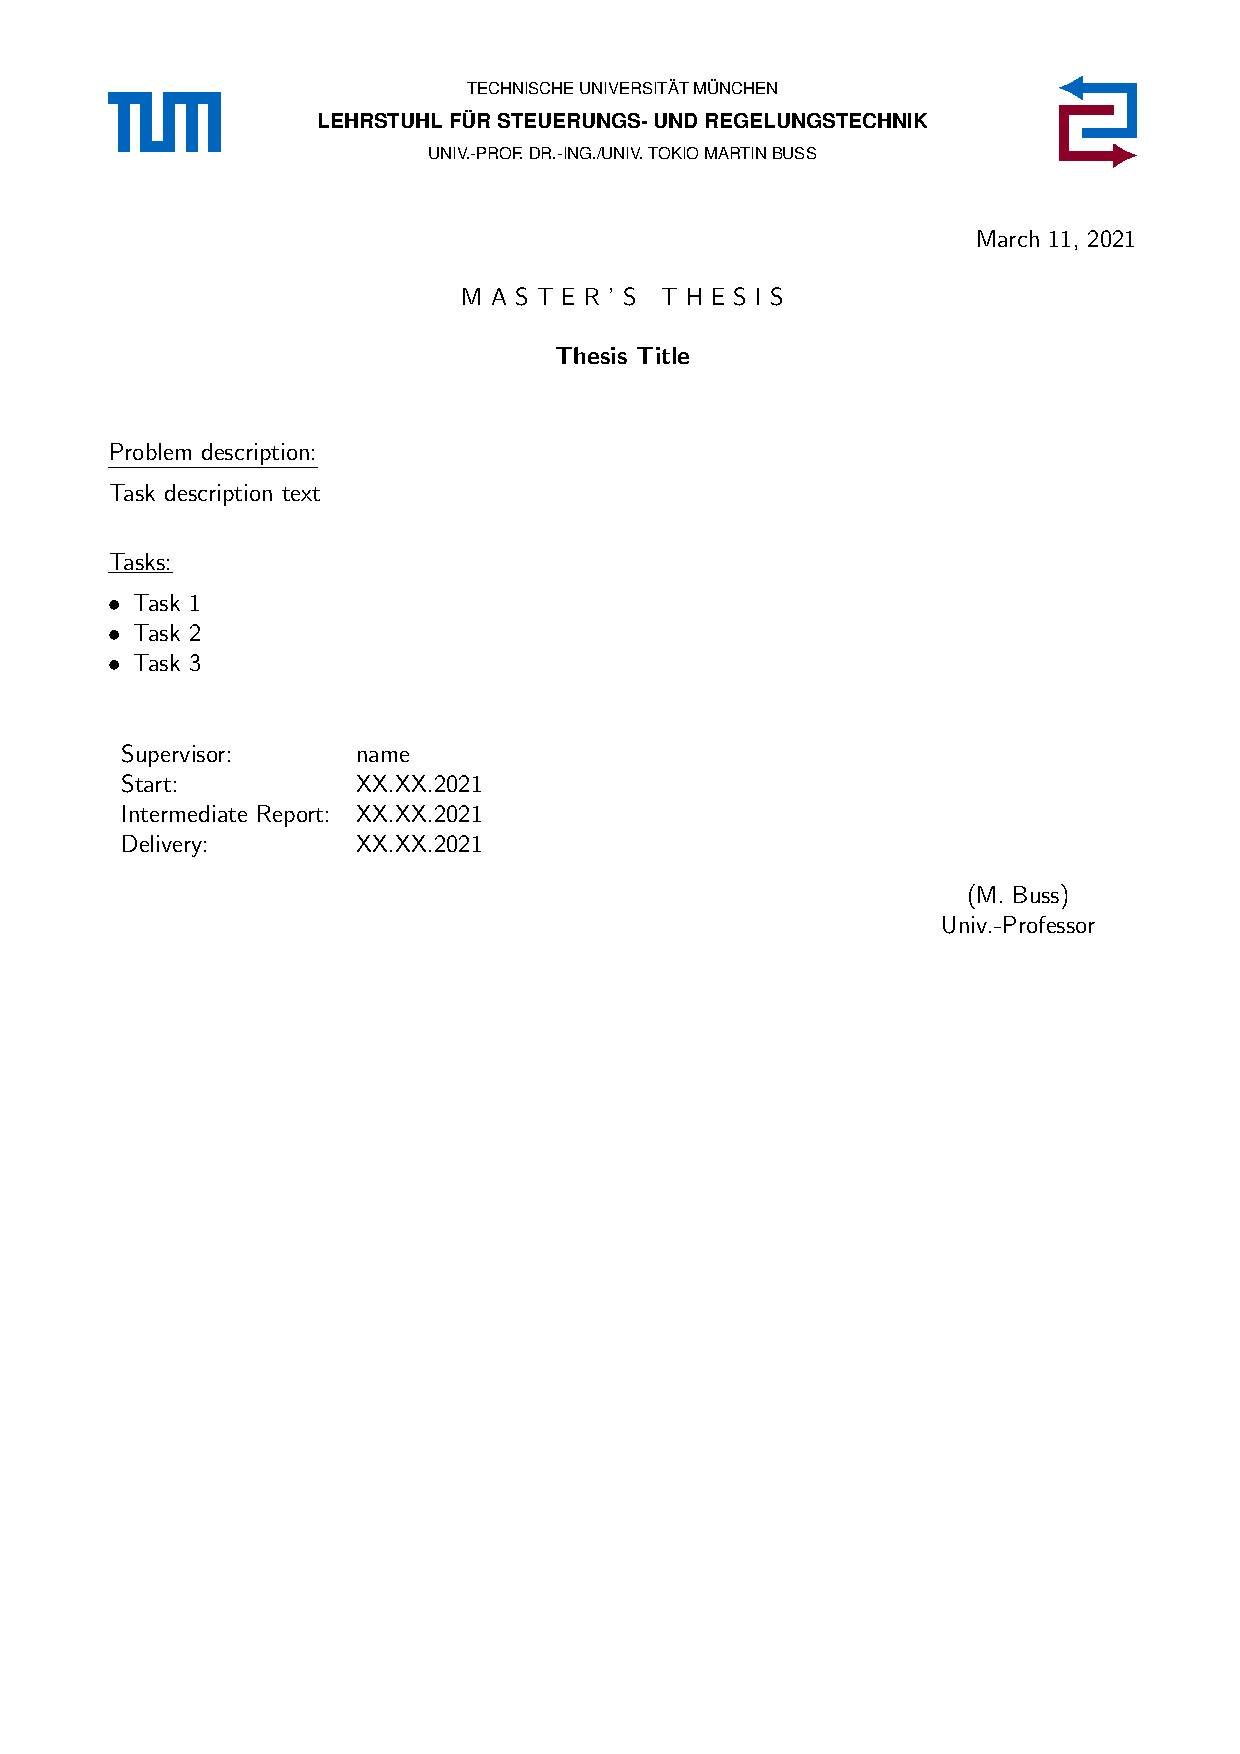
\includepdf[pages=1]{./include/task_desc.pdf}
\fi
\newpage

%%%%%%%%%%%%%%%%%%%%%%%%%%%%%%%%%%%%%%%%%%%%%%%%%%%%%%%%%%%%%%%
%%%%%%%%%%%%%%%%%%%%% abstract %%%%%%%%%%%%%%%%%%%%%%%%%%%%%%%%
%%%%%%%%%%%%%%%%%%%%%%%%%%%%%%%%%%%%%%%%%%%%%%%%%%%%%%%%%%%%%%%
\topmargin5mm
\textheight220mm
\pagenumbering{arabic}
\phantom{u}
\begin{abstract}
  A short (1--3 paragraphs) summary of the work. Should state the problem, major assumptions, basic idea of solution, results. Avoid non--standard terms and acronyms. The abstract must be able to be read completely on its own, detached from any other work (e.g., in collections of paper abstracts). Do not use references in an abstract.
%\begin{center}	
%\normalsize \textbf{Zusammenfassung}\\
%\end{center}
%Hier die deutschsprachige Zusammenfassung. 
%\optional{Talk to your supervisor if this is needed and/or wanted before starting with your thesis}
\end{abstract}
\newpage

%%%%%%%%%%%%%%%%%%%%% Widmung %%%%%%%%%%%%%%%%%%%%%%%%%%%%%%%%%
\phantom{u}
\phantom{1}\vspace{6cm}
\begin{center}
%Hier die Widmung oder leer lassen
\end{center}

\pagestyle{fancy}

%%%%%%%%%%%%%%%%%%%Inhaltsverzeichnis%%%%%%%%%%%%%%%%%%%%%%%%%%
\tableofcontents 

%%%%%%%%%%%%%%%%%%%%%%%%%%%%%%%
% ACTUAL CONTENT OF YOUR WORK %
%%%%%%%%%%%%%%%%%%%%%%%%%%%%%%%
%%%%%%%%%%%% Kapitel - externe Dateien zur Ordnung%%%%%%%%%%%%%
\ifLSRITRtutorial
	%_________Template Tutorial__________________________________

\chapter{Working with this Template}
\label{sec:Tutorial}

Please carefully read the following instructions about student reports and specifically this template. The contents of Chap.~\ref{sec:Tutorial} summarize the basics about working with this template. The subsequent chapters focus on specific parts of your report, e.g., the introduction (Chap.~\ref{sec:introduction}).

\section{General Remarks}

\optional{Please have a look at our \href{https://wiki.tum.de/display/lsritr/Students}{\underline{thesis-guidelines}} before submitting your \emph{final} thesis.}

\subsection{Revisions of your thesis}

Hand in your thesis at minimum \textbf{one week} before the deadline for correction. You will receive feedback for the final version and very likely have to do minor or major revisions of your writing. Plan your writing schedule to allow for these adjustments, which can have quite some impact on your grade! 



\subsection{Structure of your thesis}

Make sure your thesis is well structured, that each major section does what it is supposed to do, and that the overall story is clear. This template offers a common basic structure (but other structures are possible). In particular, you do not need to have exactly as many major sections or chapters as the template implies; sometimes it makes sense to merge parts, sometimes it makes sense to move parts (e.g., the location of the literature review may vary), sometimes it makes sense to split a logical part into several individual sections. Just use some common sense. 

You do not have to write down everything you do. Focus on the main results of your work and structure your report accordingly. The goal is a structured report that provides everything needed to understand and replicate your work (data, formulas, parameter values, $\ldots$). Not everything that you do/read/plot during your work has potential to be put in the report. A longer report is not necessarily better!

A sample structure is briefly provided in the following. Note again that your report does not necessarily have to follow this sample structure perfectly.

\vspace{\baselineskip}


(Sample) Structure in a nutshell:

\begin{itemize}
	\item Chapter 1: Introduction
	\begin{itemize}
			\item General motivation - understandable even to your grandma.
			\item What has been done before? (related work: How do other people solve your problem? What are drawbacks of their approaches?)
			\item How do you approach the issue? What are the challenges? What methods do you use? What is new about your approach?
			\item Describe the structure of your report: 
			\item This report is structured as follows: Chap. 2 introduces $\ldots$ . In Chap. 3 $\ldots$ . $\ldots$ is discussed in Chap. 4. $\ldots$ and so on $\ldots$
			\item Optional: put notation here.
	\end{itemize}
	\item Chapter 2: Relevant methods - describe the methods and structures you use
	\item Chapter 3: Describe your approaches
	\item Chapter 4: Simulation results
	\begin{itemize}
			\item Describe the setup/model/implementation.
			\item Give all parameters necessary to replicate your results.
			\item Show results.
			\item Discuss results thoroughly (a critical view point is important here).		
	\end{itemize}
	\item Chapter 5: Experimental results (structure similar to simulation results)
	\item Chapter 6: Conclusion
	\begin{itemize}
			\item Summarize the goal of your work.
			\item Summarize your approach and your results.
			\item Draw conclusions.
			\item Give an outlook on possible future work.
	\end{itemize}
\end{itemize}

\newpage

\section{Structuring: Sections}

Use chapters, sections, and subsections to structure your document. 

\subsection{Subsection}

This is a subsection. 

\subsubsection{Subsubsection}

Subsubsections can be used to further structure information within a subsection. They do not show up in your list of contents. Please do not use more than these two ``sub''-prefixes to sections (no: subsubsubsubsection). If you feel that you need even finer grained structuring, rethink your overall structure.

\paragraph{Paragraphs} are sometimes more useful than subsubsections to structure text without breaking the flow.


\section{Style and Expressions}

Before handing in your thesis, even for an intermediate review, please perform a spellcheck and correct grammar mistakes. Proof-read your work thoroughly BEFORE you send it to your supervisor. Text/latex editors usually have a spell check option included - use it! Be aware that latex editors often do not have the most sophisticated spellchecks.

The report is not meant to be a narrative text. Please stick to neutral and technical style and avoid subjective or biased expressions or adjectives/adverbs such as \emph{obviously, always, very, especially well, actually, so-called etc}. Scientific writing is about precision and you should underpin your statements factually, not soften them with unnecessary qualifiers. Look at the papers you read and use them as a reference on how other people write scientifically.

If you know that you often make the same errors without meaning to (e.g., use past tense, forget protected spaces, use present progressive, use a word in the wrong way, $\ldots$) in many cases the search (or replace) function helps in finding them all.

\subsection{Writing}

Choose whether you want to write American English or British English and stick with it (more common is American English). If your spellcheck allows to set dictionaries, pick the appropriate language pack (British/US) to get corrections hints that help you to consistently write in either of the two languages.
Make sure you are aware of the basic rules of English grammar (sentence structure, adverbs with ``-ly'' at the end, use of punctuation, etc.).

Keep it simple: 

\begin{itemize}
	\item Simple and short sentences (subject - verb - object)
	\item Simple words you know even if it sounds repetitive (Your teacher probably told you in school, that you should find synonyms whenever possible. You can do this when you write in your native language and you have a feeling for the words. Otherwise it is okay to sound repetitive, especially for nouns. And in any case: Do NOT just use new words without thoroughly researching all their meanings, really, don't!)
	\item If you really cannot avoid using new words, double-check whether the word really means what you want to express (translate the word back into your mother tongue and check its other meanings)
\end{itemize}

Do not use ``I'', use ``we'' instead, but do not overuse as this may sound too casual for your report. Instead use a passive form or activated objects (e.g. ``The figure shows ...'', ``The robot moves ...''). Use present tense without exceptions (especially no past tense - NEVER - not even when you write about related work or in the conclusion). Instead use simple present (``We write this in our report.'') - never present progressive (``-ing'' forms: ``We are not writing this in our report.''). Also keep in mind that punctuation is not optional. Line breaks, on the other hand, should only be used whenever a new train of thought starts. Do not overuse them. Articles (the/a/an) are also NOT optional. If you are not sure which preposition (in, on, to, $\ldots$) to use with a word, remember: Some words are used with various prepositions, but then they often have different meanings! Do not overuse ``can'' or ``cannot''. There are other formulations that often fit better.

\section{References}

Use references to your equations/theorems/figures/etc. to make it easier for the reader to follow, especially when you need it again later in a different context.
References to chapters/sections/subsections are labeled with \verb|\label{...}| and referred to with \verb|\ref{...}|. Use: 

\begin{itemize}
	\item Capital ``Chapter\verb|~\ref{...}|'' for chapters or ``Section\verb|~\ref{...}|'' for sections and subsections with protected space ``\verb|~|'' at the beginning of sentences:
	\begin{itemize}
		\item Chapter 1/Section 1.1 describes $\ldots$ .
	\end{itemize}
	\item Capital ``Chap.\verb|~\ref{...}|'' for chapters or ``Sec.\verb|~\ref{...}|'' for sections and subsections with protected space ``\verb|~|'' within sentences:
	\begin{itemize}
		\item $\ldots$ is described in Chap. 1/Sec. 1.1.
	\end{itemize}
	\item Small ``chapter'' or ``section'' (NEVER subsection, $\ldots$ - these are also sections) if it is not followed by a reference:
	\begin{itemize}
		\item In the following chapter/section, the method $\ldots$ .
	\end{itemize}
\end{itemize}

\subsection{Equations}
Refer to equations whenever it helps in understanding your text. This makes it easier for the reader to follow your train of thought:
\begin{itemize}
	\item NEVER refer to an equation before you introduce it. 
	\item Equation numbers should be put in brackets (1.1) - use\verb|~\eqref{}|, which does it automatically for you. Use the protected space ``\verb|~|'' to avoid lines starting with equation numbers.
	\item Do not start a sentence with an equation number.
	\item Do not write ``equation'' before putting the reference:
	\begin{itemize}
		\item Bad: Given Equation (1.1), it is possible to show $\ldots$ .
		\item Good: Given (1.1), it is possible to show $\ldots$ .
	\end{itemize}
\end{itemize}

\subsection{Figures}

References to figures should be included in the following way:
\begin{itemize}
	\item Capital ``Figure\verb|~\ref{fig}|'' with protected space ``\verb|~|'' at the beginning of sentences:
	\begin{itemize}
		\item Figure 1.1 shows the motion of the point mass.
	\end{itemize}
	\item Capital ``Fig.\verb|~\ref{fig}|'' with protected space ``\verb|~|'' within sentences:
	\begin{itemize}
		\item The motion of the point mass is shown in Fig. 1.1.
	\end{itemize}
	\item Small ``figure'' if it is not followed by a reference:
	\begin{itemize}
		\item The figure also shows $\ldots$ .
	\end{itemize}
\end{itemize}

\subsection{Tables}

Tables make it easy to understand the content. Less lines are sometimes better and look nicer, take a look in literature.
References to tables should be included in the following way:
\begin{itemize}
	\item Capital ``Table\verb|~\ref{tab}|'' with protected space ``\verb|~|''  at the beginning of sentences:
	\begin{itemize}
		\item Table 1.1 lists $\ldots$ .
	\end{itemize}
	\item Capital ``Tab.\verb|~\ref{tab}|'' with protected space ``\verb|~|''  within sentences:
	\begin{itemize}
		\item $\ldots$ are given in Tab. 1.1.
	\end{itemize}
	\item Small ``table'' if it is not followed by a reference:
	\begin{itemize}
		\item The table also lists $\ldots$ .
	\end{itemize}
\end{itemize}	

\subsection{Definitions / Assumptions / Theorems / Lemmas}

Basically, the same applies as for figures, tables, chapters, and sections:
\begin{itemize}
	\item Use protected spaces ``text\verb|~\ref{...}|''.
	\item Capital and full word (Definition/Assumption/Theorem/Lemma/Proposition\verb|~\ref{}|) at the beginning of sentences.
	\item Capital and short form (Def./Ass./Th./Lem./Prop.\verb|~\ref{}|) in the middle or at the end of sentences.
	\item Small and full word (definition/assumption/theorem/lemma/proposition) if used without reference.
\end{itemize}

\section{Equations}
Include equations in your text in a meaningful way. Example: 

\vspace{\baselineskip}
\fbox{\parbox[c]{\textwidth}{

The equation of motion of a point mass is given by 
\begin{equation} m \ddot{x} = f \ , \label{eq:motion} \end{equation}

where~$m\in\mathbb{R}$ is the mass,~$f\in\mathbb{R}$ the externally applied force, and~$\ddot{x}\in\mathbb{R}$ the acceleration in~$x$-direction.}}

\vspace{\baselineskip}

You can use~\eqref{eq:motion} to reference an equation in the
text. Equations without reference number:
\[
y=x^2
\]



Please type all numbers in mathematics mode.
Mathematical equations that are not part of the text should be centered. If you have multiple lines with equations, align equations with the arithmetic operator \verb|(=,<, ...)|:
\begin{subequations}
\begin{align}
a &= 2\\
b&= 3+4
\end{align}
\end{subequations}
Type physical units as normal text, e.g., s, not $s$! (the package \textit{siunitx} helps)
Formulas must not jut out over the text margin, so take care to stay within the margins and eventually break the equation into several lines.
Explain the variables you use. For each newly introduced variable, at least a short description of the variable should follow the equation in the style of \emph{\ldots with $x$ being the position of the cart and $u$ the control input.} Use variable names whenever possible to make it easier for the reader to make the connection: 
\begin{itemize}
\item[-] Bad: A high mass slows down the acceleration. 
\item[-] Good: A high mass~$m$ slows down the acceleration.
\end{itemize}
A parameter or variable must not be used at the beginning of a sentence.
Mathematical units must be consistently labelled with only one variable. \hl{Do not
use a variable for more than one mathematical unit}.

If you use in-line equations, either to introduce parameters or for actual equations, put a ``\verb|~|'' in between the in-line equation and the preceding word. This is a protected space - it avoids that the equation is moved to the next line, which would be considered bad style. 

If you use descriptive text in equations, set it as \verb|\text{}|. Examples:
\begin{itemize}
	\item $x_{\text{measured}}$: ``measured'' is descriptive here and not a variable/parameter 
	\item $q_{\text{des},i}$: ``des'' is descriptive here but ``$i$'' is a counter and therefore not in text 
\end{itemize}

If you want to generate more sophisticated equations, use the \textit{IEEEtrantools} package. 
%, which is used as follows:
%\begin{IEEEeqnarray}{r c l}
%\IEEEyesnumber
%a =& b &= c \IEEEyessubnumber \\
%c =& d+e &= 5 \IEEEyessubnumber
%\end{IEEEeqnarray}
This package is especially useful if custom spacing is required for multiple equation lines.

\subsection{Notation Consistency}

Consistency is key: Choose a style for your notation and stick with it. We suggest giving a notation list somewhere in your report (ideally in the beginning). 
Most often used:
\begin{itemize}
	\item vectors: bold, small letters \verb|\mathbf{}| ($\mathbf{a}$) or \verb|\boldsymbol{}| ($\boldsymbol{a}$)
	\item matrices: bold, capital letters \verb|\mathbf{}| ($\mathbf{A}$) or \verb|\boldsymbol{}| ($\boldsymbol{A}$)
	\item scalars: small (sometimes also capital), non-bold letters ($a$)
	\item general sets: \verb|\mathcal{}|
	\item sets of numbers (real, whole, $\ldots$): \verb|\mathbb{}| ($\mathbb{A}$)
\end{itemize}

\subsection{Symbol Glossary}

Instead of writing mathematical symbols individually in each equation, you can also use a glossary entry. For example, instead of explicitely writing \verb|\mathbf{u}_k| to denote a control input $\mathbf{u}_k$ at time step $k$, you can define a glossary entry, e.g., ``uk'', and just use \verb|\gls{uk}|, which then also yields \gls{uk}. Glossary entries for symbols are defined in the file ./include/gloss.tex.

This procedure is useful for two reasons: 1) You can shorten long symbol expressions significantly. 2) If you later want to change a symbol, you only need to change the glossary entry once - you don't need to change every single symbol in your document.

\subsection{Style Notes}

There are a few important style notes to consider in equations.
\begin{itemize}
\item Indices: Use italic font for math-related indices (parameters, variables, ...) and non-italic font for other descriptions, e.g., $x_t$ (time $t$) and $x_{\text{ref}}$ (ref: reference).
\item Mathematics operations are non-italic, e.g., $\sin(x)$. Often, functions are already defined in latex (e.g., use \verb|\sin(x)|). If not, use \verb|\mathrm{}|, e.g., $\mathrm{sin}(x)$.
\item Make sure parentheses are large enough by using \verb|\left( . \right)|, e.g., \[\left( \frac{1}{2} \right) \textnormal{instead of } ( \frac{1}{2} ) .\]
\item Use \verb|^\top| for a transpose, e.g., $\boldsymbol{x}^\top$.
\end{itemize}



\section{Figures}

For pictures, you can use .pdf, .jpg, .png, etc when working with \textbf{pdflatex}; with \textbf{latex} you need .eps:
\begin{figure}[htb]
\centering
%\includegraphics[width=0.2\textwidth]{lsr_logo}
%\includegraphics[width=0.9\textwidth]{abbildung.eps}
\caption[Abbreviated Description]{Long Description: The subtitles of tables and illustrations should be self-explanatory.}
\label{fig:abb1}
\end{figure}

Figures should be vector graphics (pdf or eps) and self-made (to avoid blurry pictures). We recommend pgfplots/tikzpiktures or inkscape and Matlab (export figure with tick set at Rendering - Custom renderer: painters) in combination with \verb|\psfrag{ }[ ][ ]{ }| to replace the text in \LaTeX.

Every illustration must be described and referenced in the text, cf. Fig. \ref{fig:abb1}. 
There is no such thing as a decorative figure! 
If the figure is not mentioned in the text and therefore lacks an explanatory function, leave it.
Lines in plots need to be clearly distinguishable, also in black-and-white print. Therefore, choose your colors and line styles wisely and consistently!
The subtitles and axis labels must be clearly legible (i.e., big enough) and include a scaling. Ideally, the figure is self-explanatory with labels, arrows, text, etc. Text in figures should be without serif: \verb|{\sf your_text_goes_here}|, about the same size as the ``normal'' text and labels should include all important information such as the name of the depicted variable and the corresponding unit. Captions should clearly describe the content. If the caption is rather long, use ``\verb|\caption[short_caption]{long caption}|''. The long caption appears below the figure, the short caption appears in the list of figures. 

Figure axes need to be labeled correctly. Do not just mention the variable name but include a description. If units are required, use parenthesis. An example is given in Fig.~\ref{fig:vel_plot}.

\begin{figure}[htb]
\centering
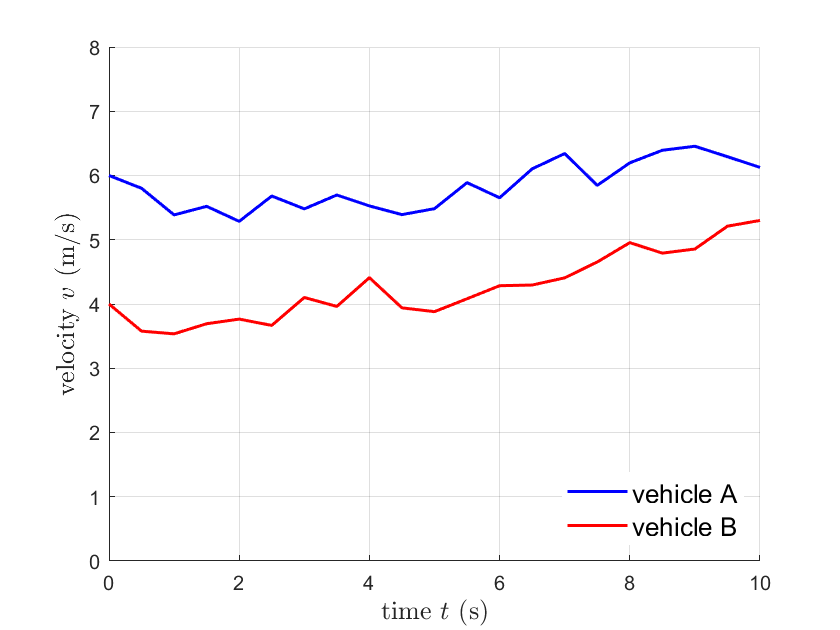
\includegraphics[width=0.6\textwidth]{pics/velocity_plot.png}
\caption{Example velocity plot with units}
\label{fig:vel_plot}
\end{figure}

If the illustration is copied from another person's work, you need to mention the
source with \verb|\cite{}|.

By using \textit{subfigure}, several pictures can be combined in one main picture as in Fig.~\ref{fig:OverallPic}:

\begin{figure}[htb]
\centering
\subfigure[Subfigure 1 caption]{
   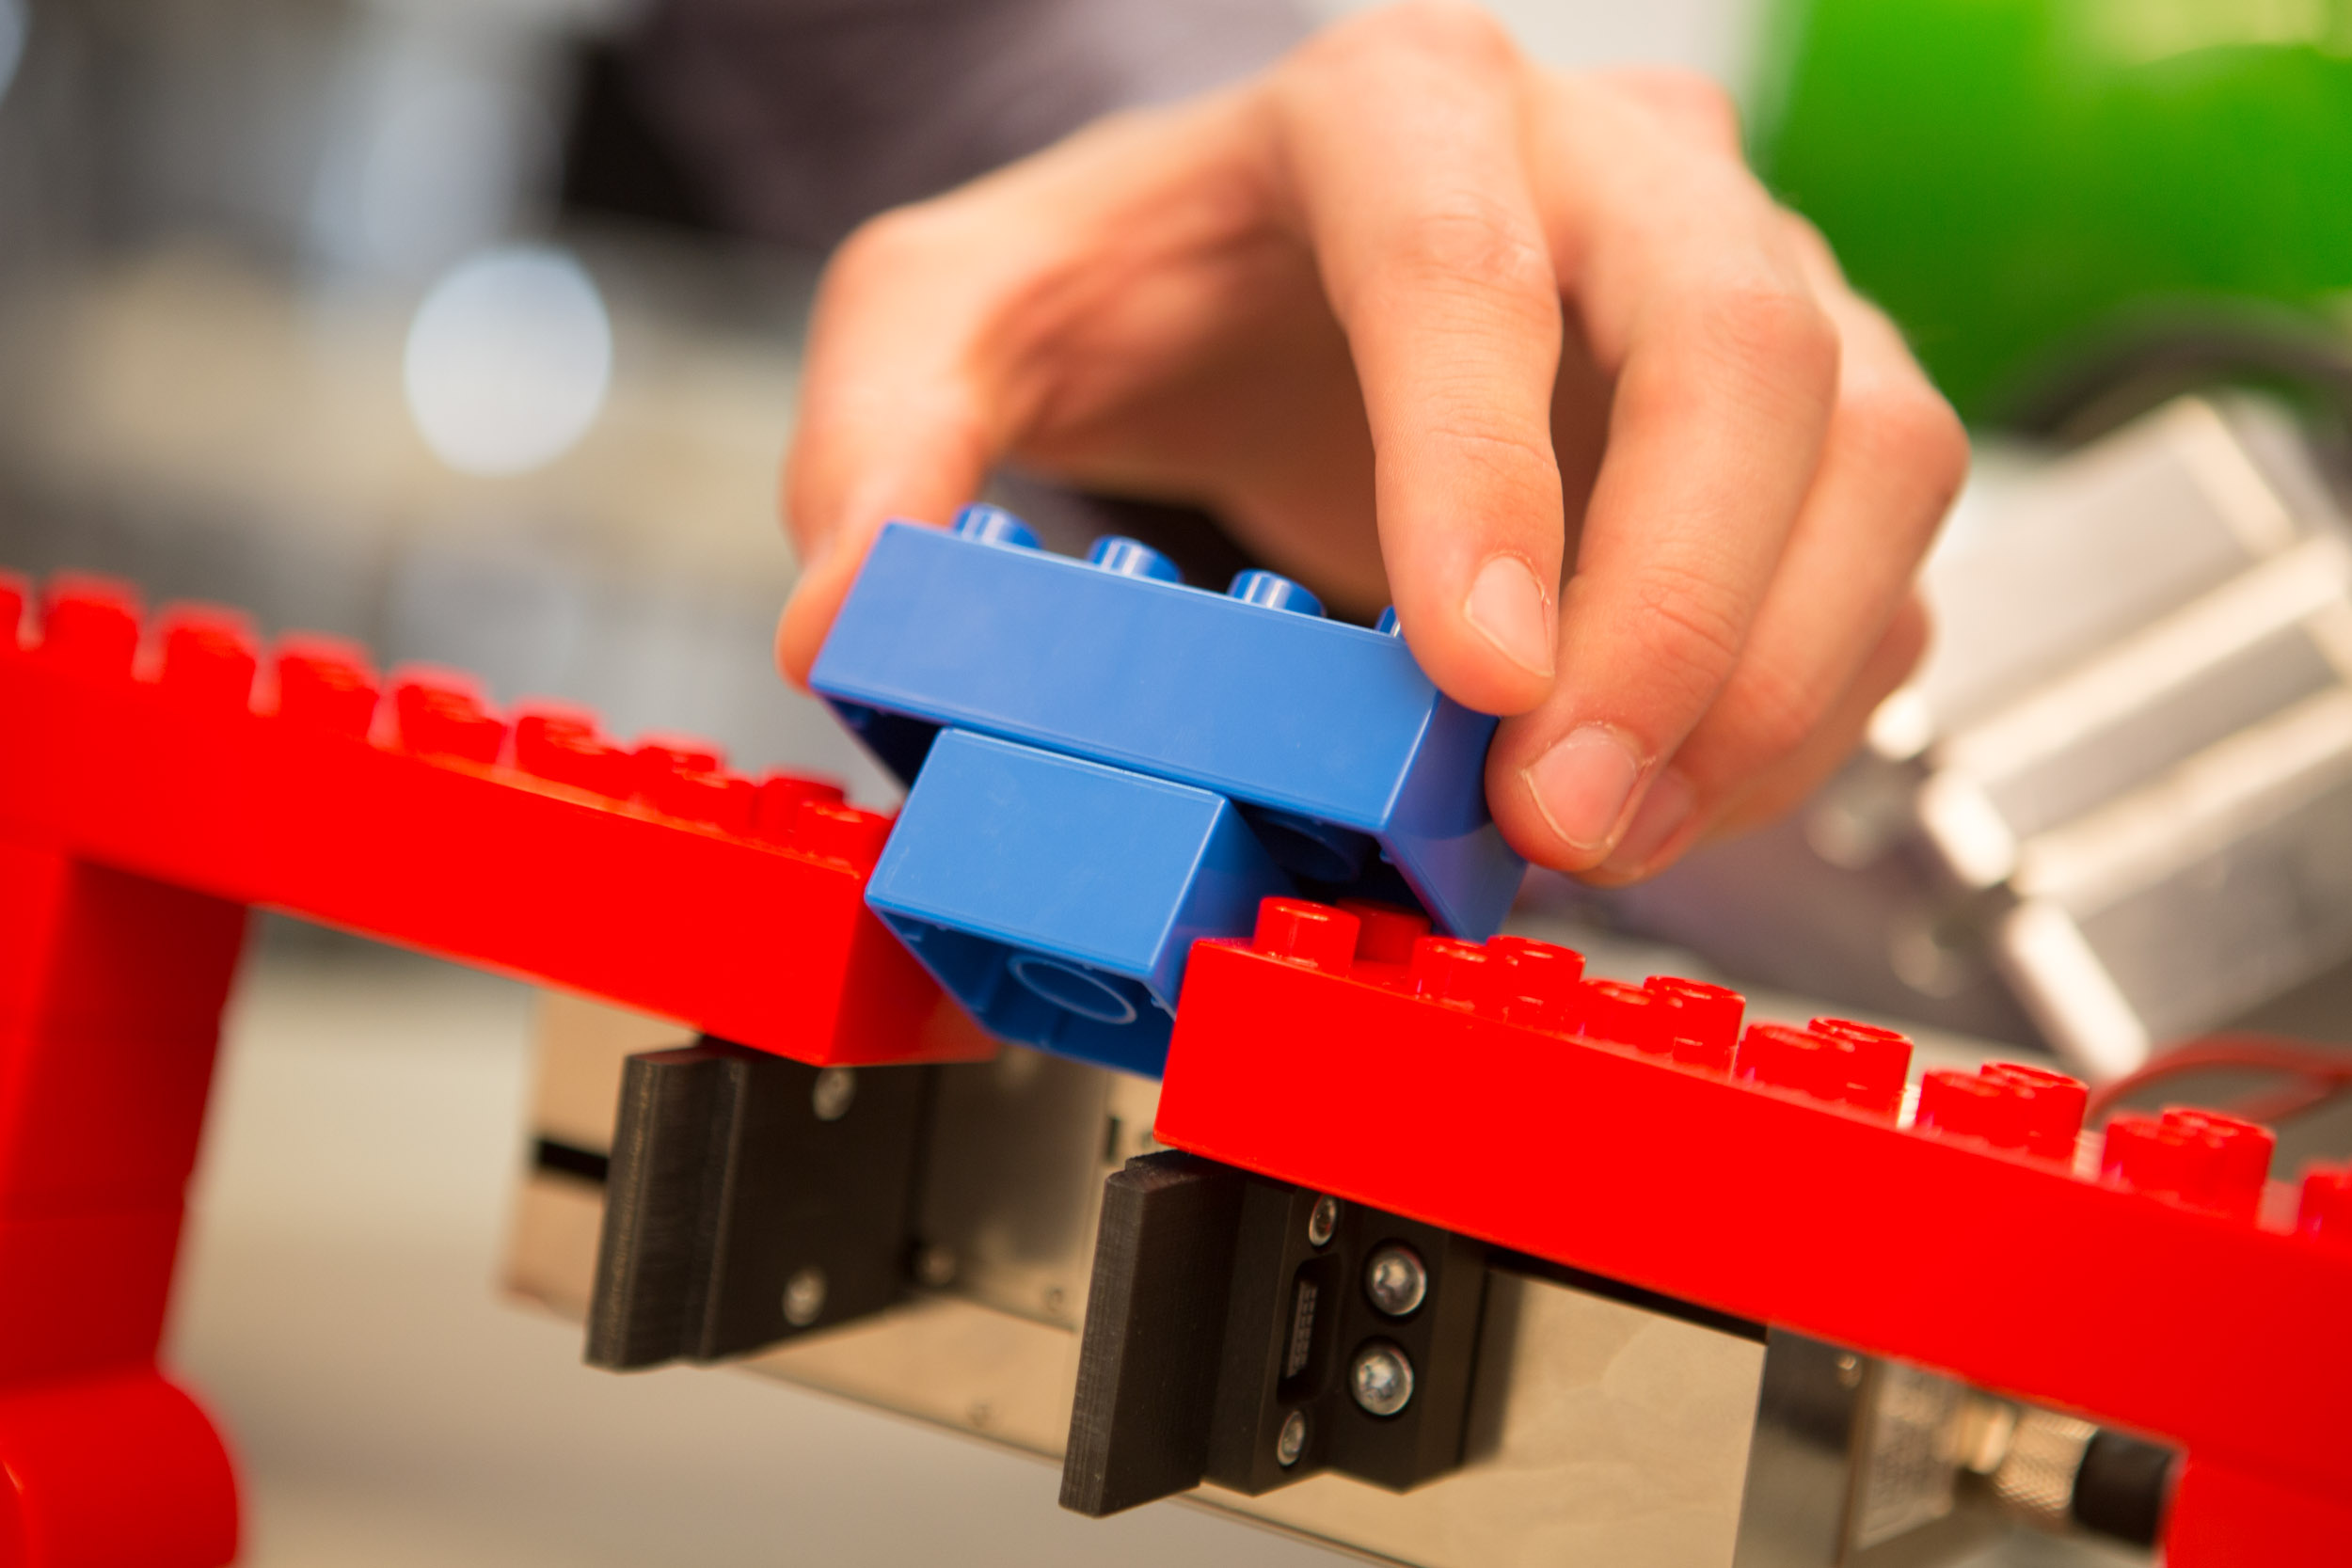
\includegraphics[width=0.3\textwidth] {Lego_robot3}
   \label{fig:subfig1}
 }
\quad % puts next subfigure right next to the previous subfigure
\subfigure[Subfigure 2 caption]{
   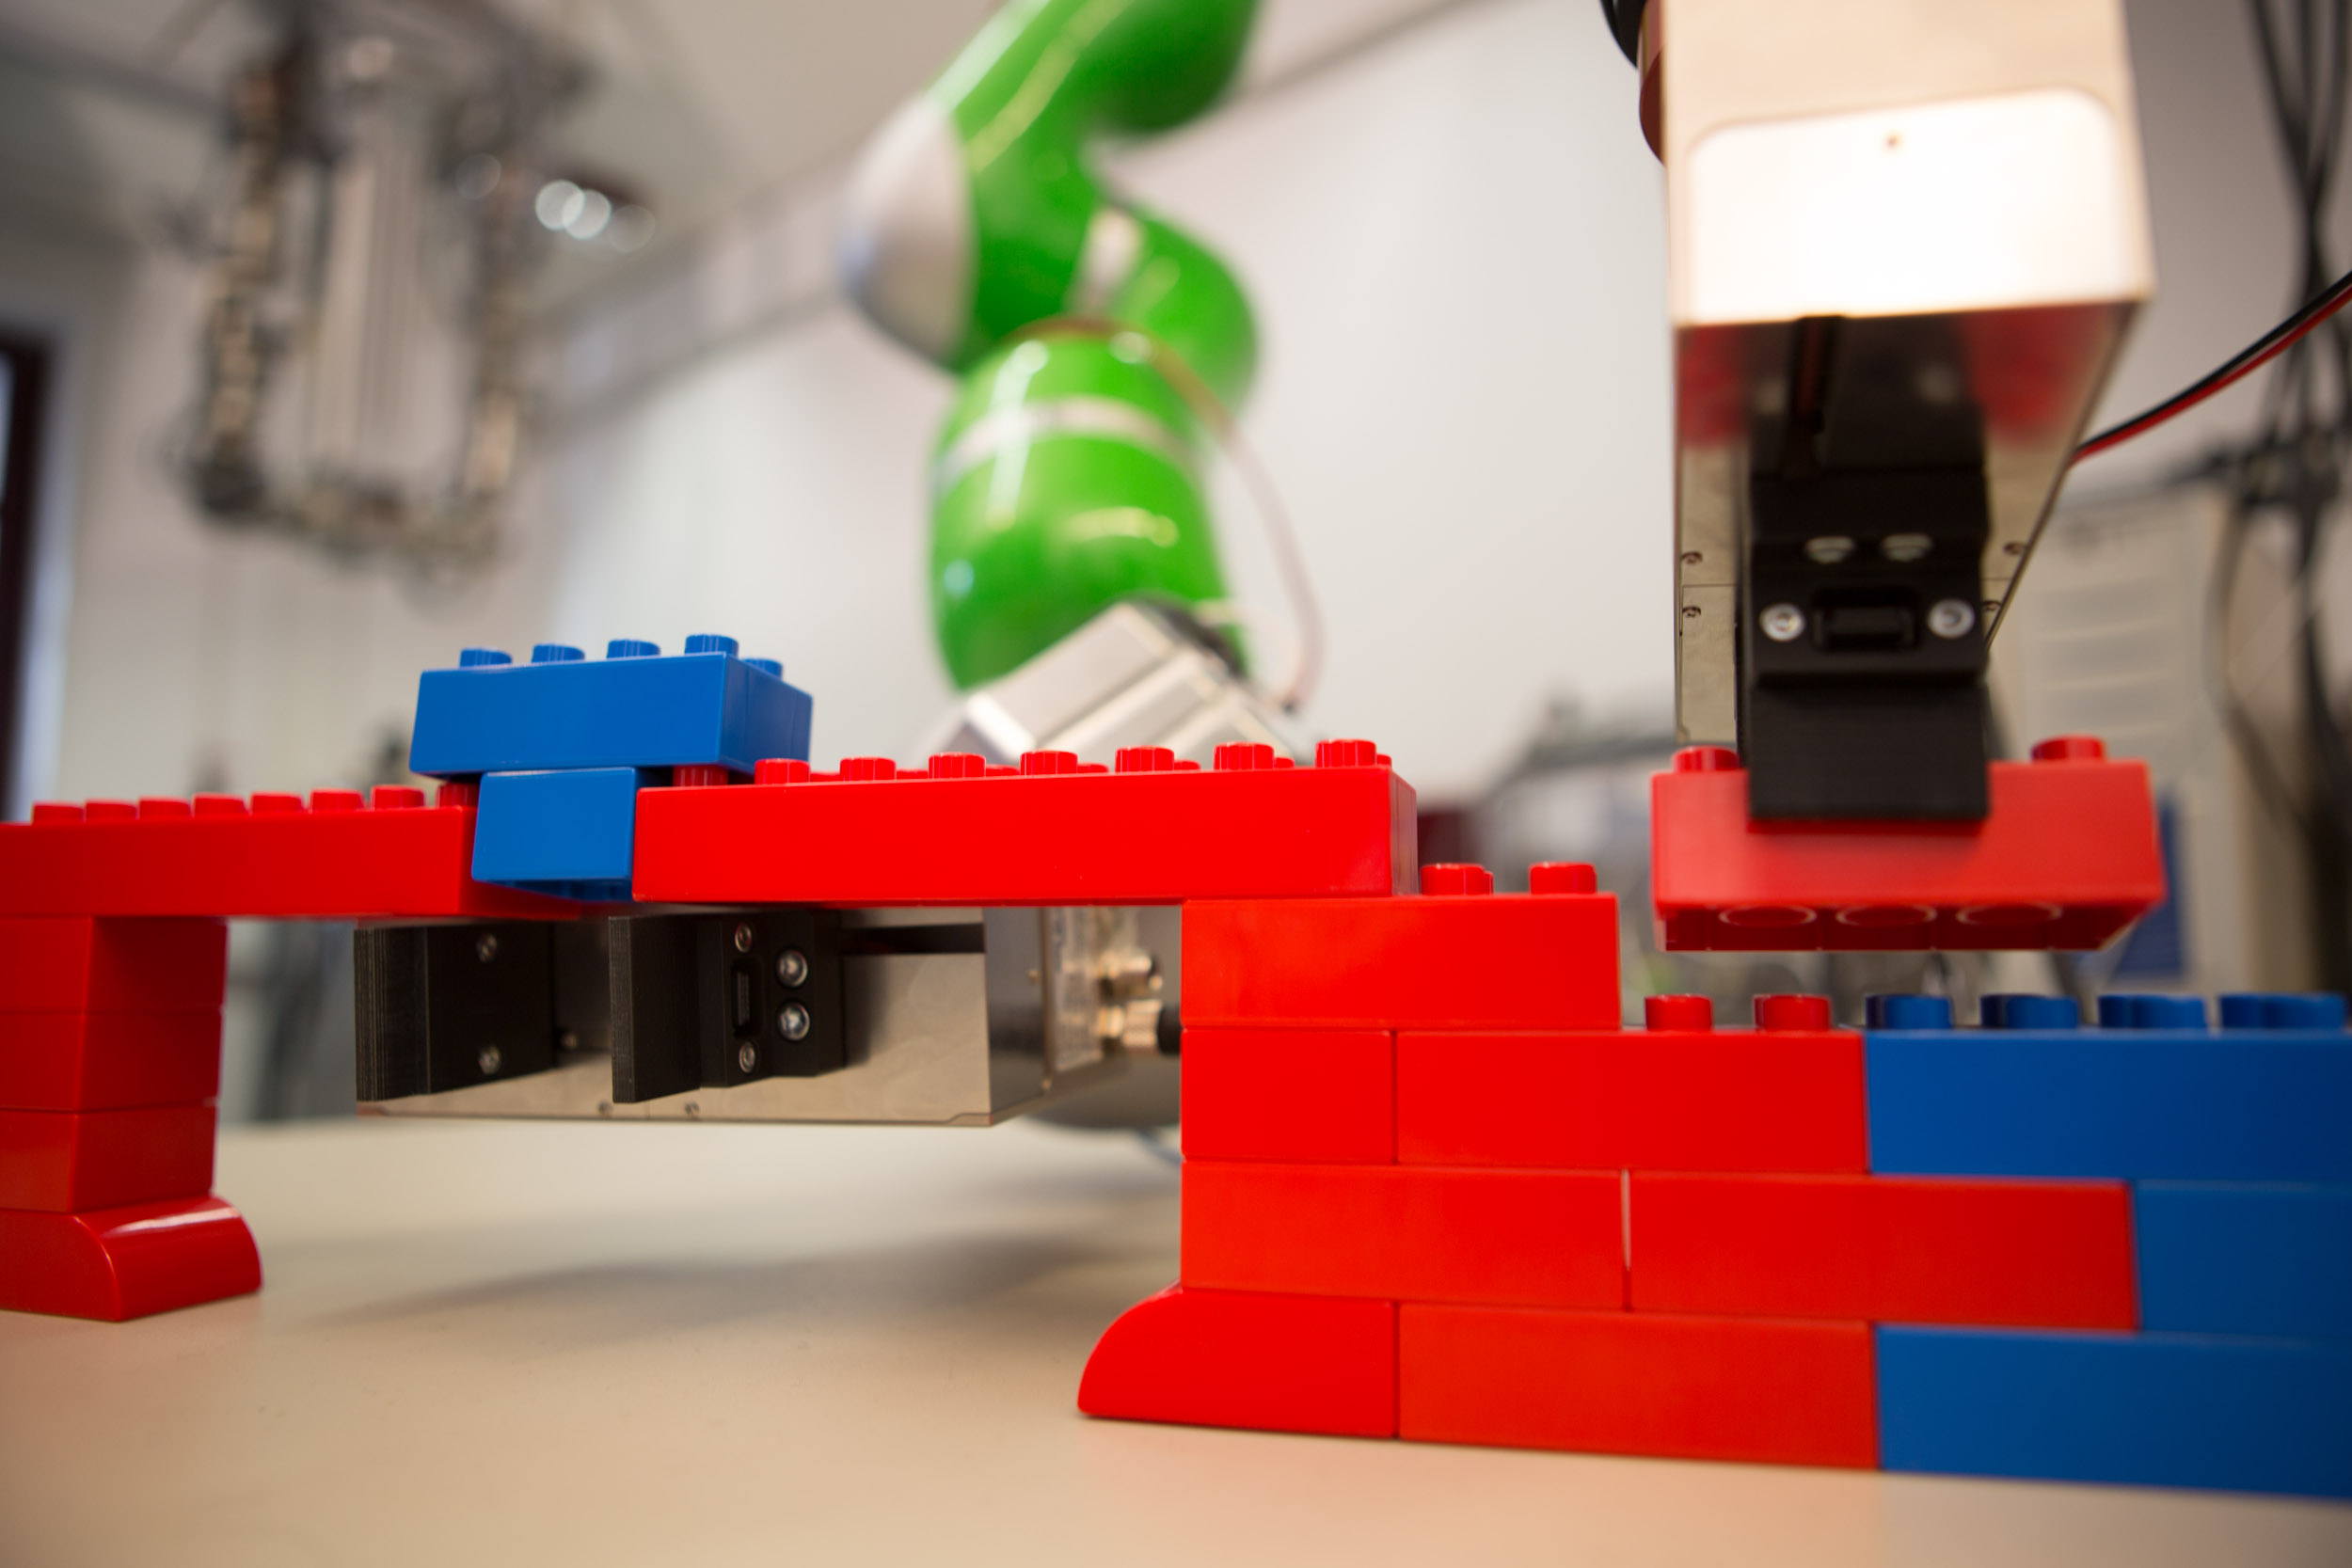
\includegraphics[width=0.3\textwidth] {robot_build}
   \label{fig:subfig2}
 }

\subfigure[Subfigure 3 caption]{
   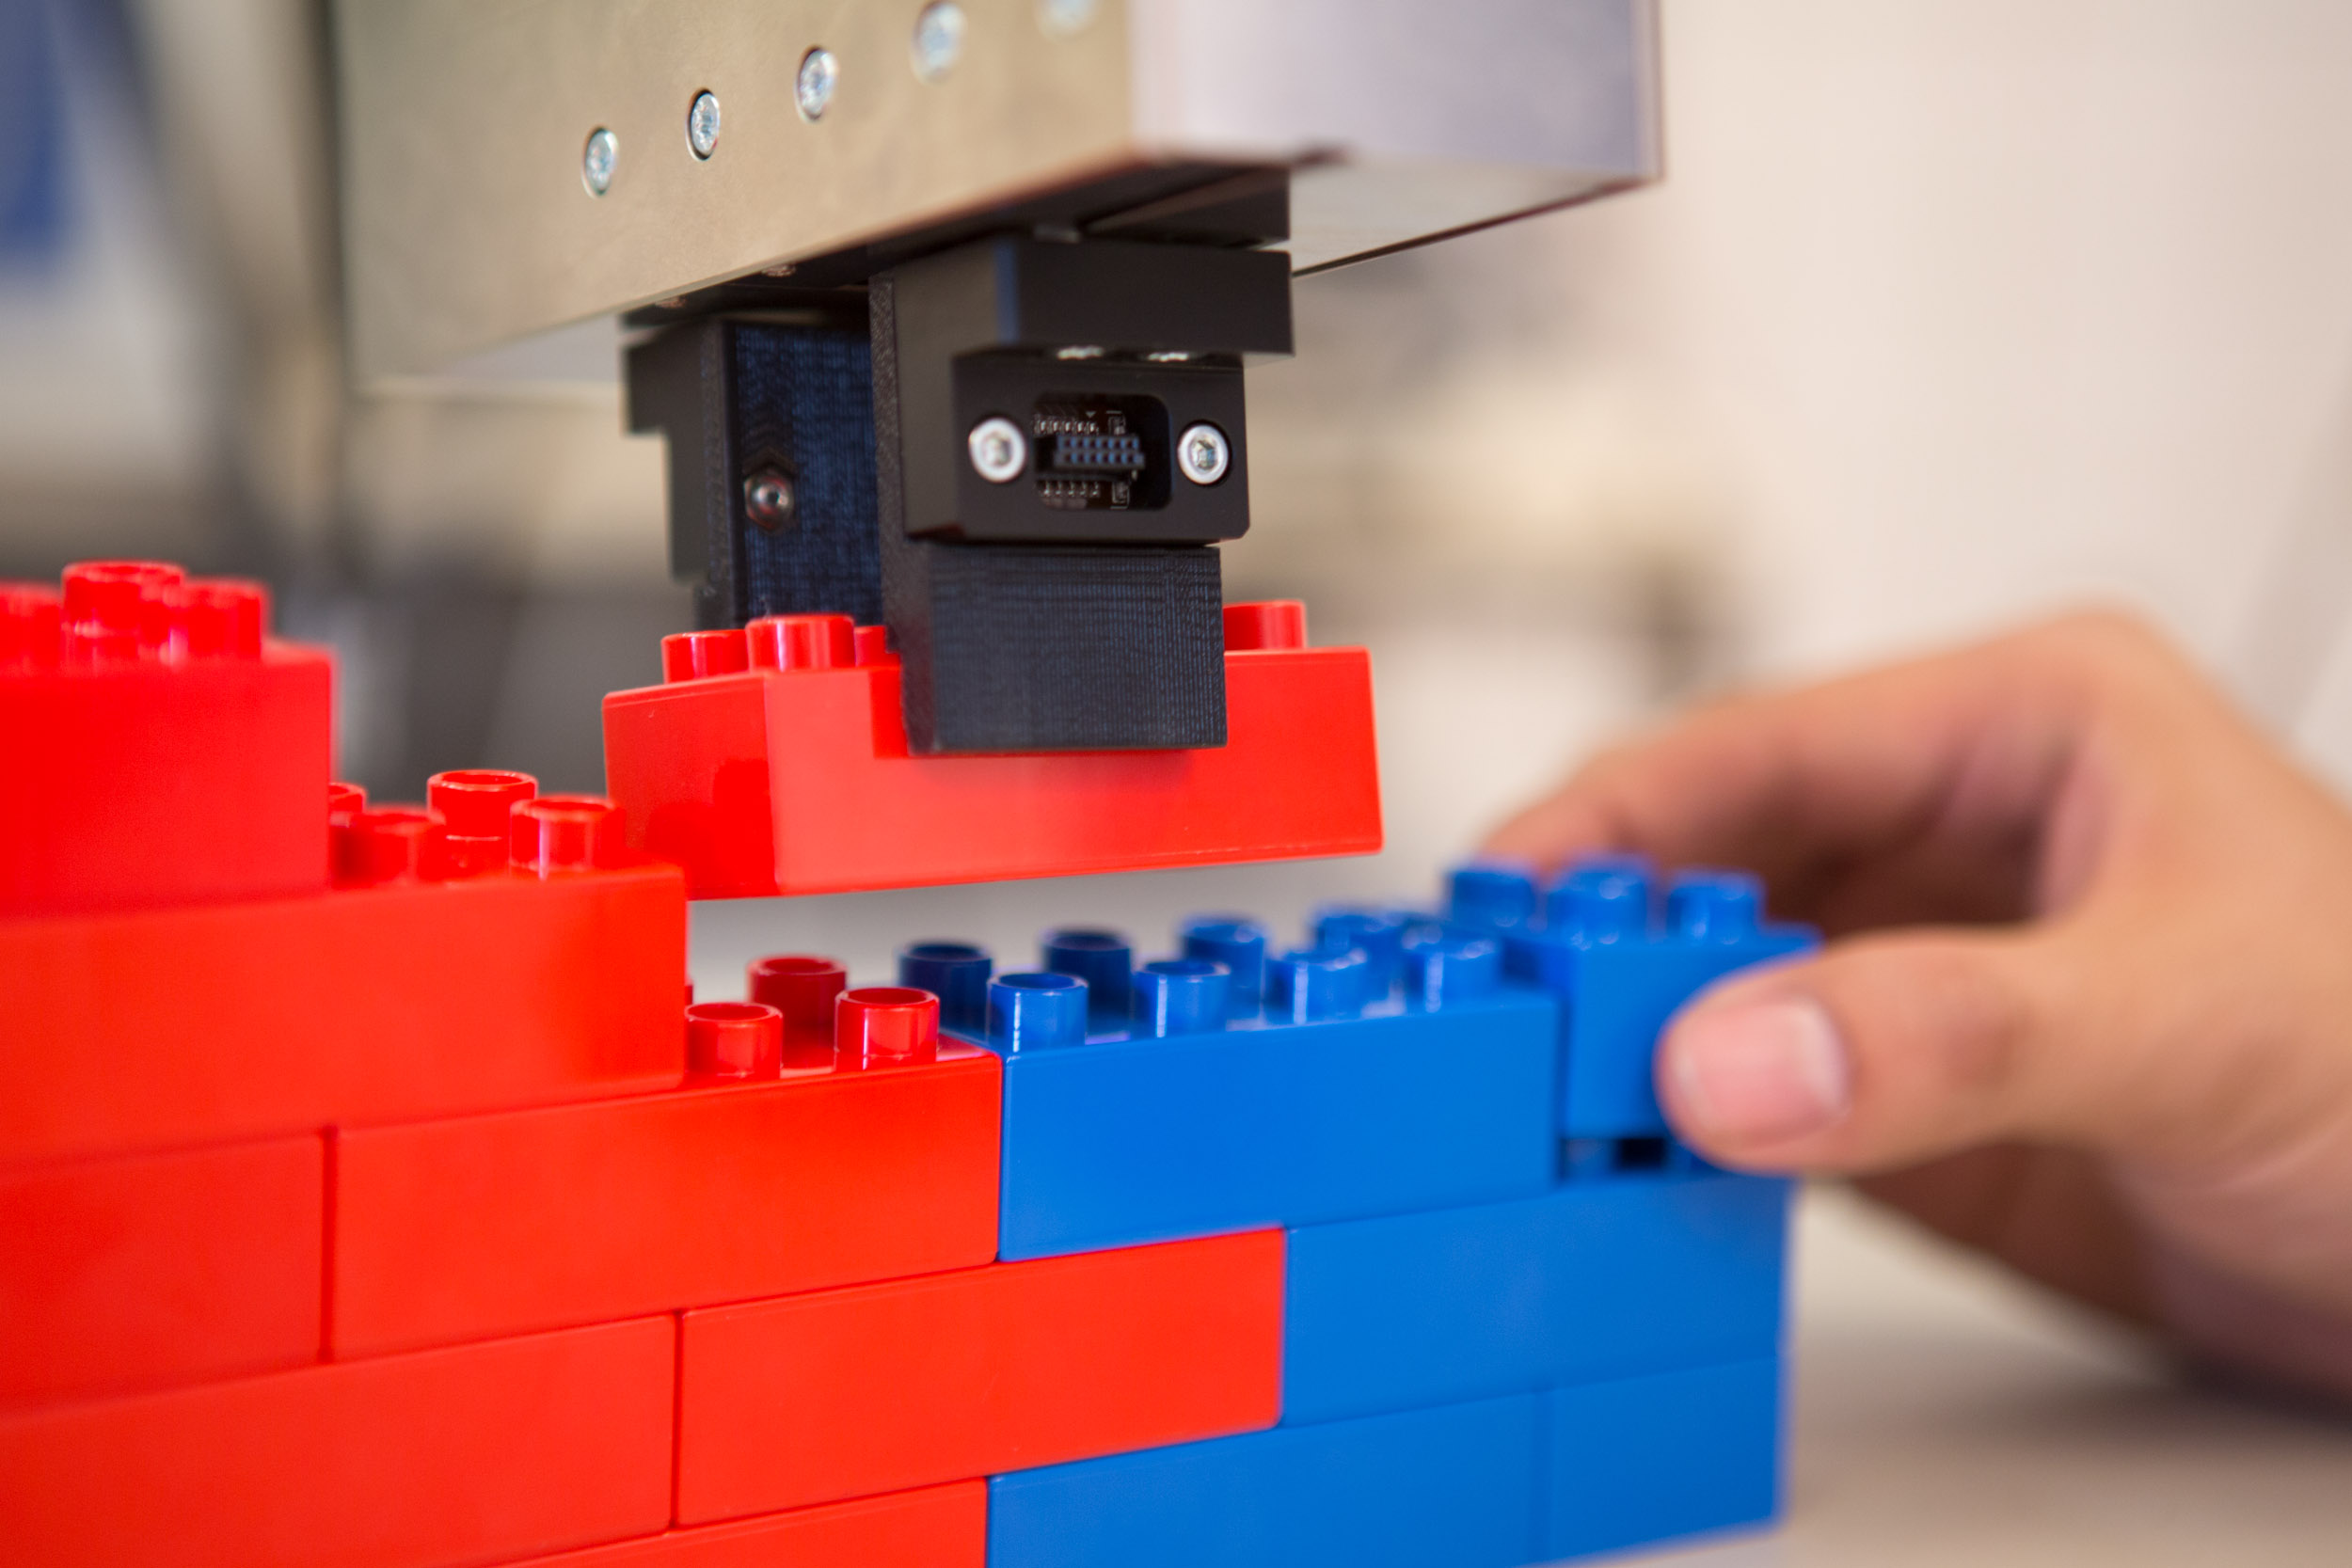
\includegraphics[width=0.4\textwidth] {robot_build_withHuman}
   \label{fig:subfig3}
}
\subfigure[Space-holder for missing picture]{
	\missingfigure[figwidth=0.4\textwidth]{
		\tiny{A Picture needs to be  put here later. One can use acronyms, e.g. \acs{HRC}}}
	\label{fig:subfig4}
}  
\caption[Abbrev. Descr. of subfigure-figure]{A figure with two subfigures}
\label{fig:OverallPic}
\end{figure}

This figures can be referenced by either referencing the overall label \ref{fig:OverallPic} or a specific subfigure label \ref{fig:subfig1} - if the labels have been set properly of course! The subfigures are not listed in the list of figures!



\section{Definitions / Assumptions / Theorems / Lemmas}

Sometimes a definition is helpful, especially for later reference. Motivate and introduce each one and do not just list definitions one after another. Explain why it is important and what it is used for. Assumptions are useful to emphasize what preliminaries have to be fulfilled for your approach to work, especially if you plan to introduce theorems, lemmas, etc. 

Points to remember:
\begin{itemize}
	\item Do not list assumptions one after another. 
	\item Motivate and introduce each one.
	\item Explain how restrictive it is and illustrate its effects on the application.
\end{itemize}

Sometimes you need to cite a theorem/lemma/proposition. 

Points to remember:
\begin{itemize}
	\item Same as above: do not just list, motivate, introduce, explain what this enables.
	\item Make yourself familiar with the way theorems/... are usually formulated. Look at the literature. 
	\item Make sure all relevant assumptions and preliminaries are stated in the theorem/...
	\item Make the proof (if it is your own theorem/...) conclusive and understandable.
\end{itemize}



\section{Citations}

Citations are extremely important and \textbf{must} be included whenever you use other people's work. Direct citations with directly copy-pasting the content and marking it with ``$\ldots$'' are unusual in scientific reports. Always try to reformulate the source into your own words to generate an indirect citation. 


Whether to use numeric or alphabetic references is not all that important (unless prescribed by a conference or journal), but alphabetic tends to be more readable. Independent of citation style, the following rules should be followed:

\begin{itemize}
\item Use the \LaTeX~cite package. It does not give you additional commands, but it fixes a few quirks in \LaTeX. Among others, it automatically sorts multiple citations, and it correctly spaces the angular brackets (if you use the \verb|\cite{}| command without leading white space).

\item Citing several papers at one point should be done with a single \verb|\cite{}| command. For example, use \verb|gives good results\cite{Bloe_99, Jay_87}|, resulting in gives good results \cite{Bloe_99, Jay_87}. 

Do not use \verb|gives good results\cite{Bloe_99}\cite{Jay_87}|, which produces the ugly gives good results \cite{Bloe_99}\cite{Jay_87}. Also, note that there is no space between the \verb|\cite{}| command and the preceding word, \LaTeX~(with the cite package) does the spacing correctly.

\item Avoid citations of the kind: \cite{Bloe_99} thinks that $x>y$ is valid, but \cite{ONeill_2000} argues that this is invalid in case of $z\geq5$. This works a bit better if using alphanumeric citation labels. Better, though, use the authors' names: Bloe and Joe [1] think that $x>y$ is valid, but O'Neill et al. \cite{ONeill_2000} argues that this is invalid in case of $z\geq5$. 

\item Avoid citations at the beginning of a sentence:
	\begin{itemize}
		\item Bad:
		\begin{itemize}
			\item \cite{Bloe_99} introduces different methods for motion control. (citation at the beginning)
			\item Different methods for motion control are introduced in literature. \cite{Bloe_99} (citation after the punctuation)
			\item Different methods for motion control are introduced in\cite{Bloe_99}. (preceding space missing or wrong cite package)
		\end{itemize}
		\item	Good: 	 
		\begin{itemize}
			\item Different methods for motion control are introduced in \cite{Bloe_99}.
			\item Khalil et al. introduce different methods for motion control \cite{Bloe_99}. 
			\item Motion control as in \cite{Bloe_99} is generally used to $\ldots$ .
			\item Motion control \cite{Bloe_99} is generally used to $\ldots$ .
			\item Motion control is generally used to $\ldots$ \cite{Bloe_99}.
		\end{itemize}
	\end{itemize}


\item BibTeX is a great tool, but you need to know how to use it. A regular trap is to forget that \TeX~knows more about typesetting than you do. So, for example, it changes the case of words in the title. If your title contains acronyms and proper names (most do), they tend to get down-cased. Any such words which should not have their case changed should be put into braces, e.g., \verb|{The {Mungi} {OS} and its Use in Merry-Go-Round Seat Allocation}|.


\item In citations do not abuse the category technical report. People tend to cite just about anything that has not been published in a journal or conferences as a TR. This is outright wrong. The concept of a TR is actually fairly well defined: A TR is published in some sort. This is generally as part of a formal TR series of some institution, in hardcopy or on the web or both. (They are not always called ``technical report'', other common names are ``research report'', ``technical memorandum'', $<$institution$>$ ``report'' etc.) The publication (i.e., availability outside) is essential, otherwise it's at best an internal report.
A TR has a number (absolutely!), an institution (publisher), a date (month and year at least) and a publisher's address (besides all the other stuff bibentries have).
If your document doesn't have these features, it's not a TR. It is probably better categorized as a working paper. Even then it has a date and an institution address.

\item Citing web pages is often unavoidable (but also often a sign of laziness). When citing web pages be aware that they may only be short-lived. Consider whether the reference will be of any use to the reader at all if the link is broken. Or whether your whole document only has a use-by date a few months past writing.

\end{itemize}

Any cited document, whatever it may be, has a few \textbf{mandatory} features:
\begin{itemize}
	\item Date. Absolutely. 
	\item Author/organization/creator/person responsible for contents.
	\item Whatever information the reader needs to find that document. In most BibTeX entry types these are clearly identified as mandatory fields. Mandatory means that they aren't optional. Do not pretend they are. For a working paper these might be the contact details of the author.
\end{itemize}


For bibliography, edit {\tt mybib.bib} and list all
references in a special style, e.g., for a book: 
\begin{verbatim}
@book{literaturstelle1,
 author    = {S. Sastry},
 title     = {Nonlinear Systems - Analysis, Stability, and Control},
 publisher = {Springer},
 year      = 1999
}
\end{verbatim}

Cite references in the text by \verb|\cite{citationreference}|.

In order to have your references shown in your PDF, compile by:

\begin{verbatim} 
latex myfile
bibtex myfile
latex myfile
latex  myfile
dvips myfile
ps2pdf -sPAPERSIZE=a4 myfile.ps
\end{verbatim}

Alternatively you can use your preferred \LaTeX -editor. The according BibTeX compiler has to be configured properly and then run before running PdfLaTeX. We recommend you to use our preconfigured editors.

\hl{Make sure your bibliography is consistent (e.g., all first names abbreviated).}

\section{Compiling}
Linux: 
do the following in a Shell:\\
\begin{verbatim}
latex myfile
dvips myfile
ps2pdf -sPAPERSIZE=a4 myfile.ps
\end{verbatim}
Make sure to use the A4 option, when you print the pdf!

Alternatively you can use either Kile, Texmaker, etc. on Linux or TeXnic Centre, etc. on Windows. Please be aware you have to set the required \LaTeX paths in your editors. The most common \LaTeX -editors in Linux are preconfigured at LSR and should work \emph{out-of-the-box}.





\fi
%_________Einleitung__________________________________
\chapter{Introduction}
\label{sec:introduction}

MPC is a control technique that uses models of the plant in order to predict the future behaviour of the system over a prediction horizon. Usually, these models are expressed mathematically as ordinary differential equations (ODE) \cite{sanchez2017mpc}. Applying MPC schemes to continuous time systems requires numerical
discretization of the continuous time optimal control problem. Commonly used discretization approaches for MPC are based on RK methods. For the implementation in a sampled control loop, typically zero-order hold (ZOH), i.e., piecewise constant inputs between the sampling intervals are used. In applications where the continuous time model is exactly known and high accuracy control is required, a finer discretization grid or a higher order RK method can be chosen to decrease the
approximation error of the discretization method, e.g., Gauss collocation \cite{kotyczka2021high} with appropriate higher-order hold elements.

\section{Problem Statement}

 The goal of this work is to derive a trade-off between prediction accuracy and computational complexity within an MPC scheme for continuous time linear systems. This is investigated by varying the granularity of numerical discretization and the order of RK methods, including the order of the hold element in the sampled control loop. In addition, the effects of the discretization approaches on the computation of reachable and invariant sets are also examined. Results from this work will enable similar investigations for the sampled control of continuous time nonlinear systems by MPC schemes.  In MPC, higher accuracy of the discretization leads to increased computational load as more decision variables are introduced to the optimal control problem, which can result in infeasible computation time.



%____________________________________________________
\chapter{Technical Approach}
In the following, we will discuss methods on how to retrieve a discretized system of the form (4) from a given contunuous-time system equation as in (3). During the analysis of different discretization methods, we firstly introduce the zero-order hold (ZOH), i.e., piecewise constant inputs $u$ between the sampling intervals $\Delta t$, and first-order hold (FOH), i.e., piecewise linear inputs $u$ between the sampling intervals $\Delta t$. The ZOH is illustrated in Fig. \ref{fig:ZOH} and FOH is illustrated in Fig. \ref{fig:FOH}
\begin{figure}[h]
	\centering
	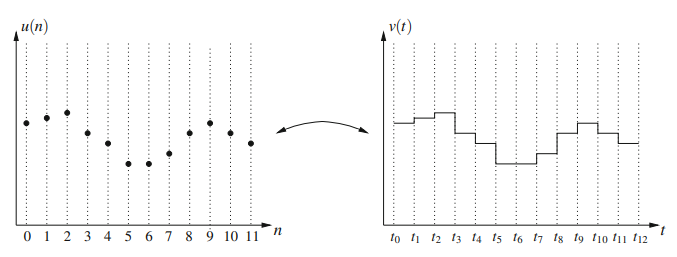
\includegraphics[width=\linewidth]{pics/ZOH.png}
	\caption{Illustration of zero-order hold \cite{grune2017nonlinear}}
	\label{fig:ZOH}
\end{figure}
\begin{figure}[h]
	\centering
	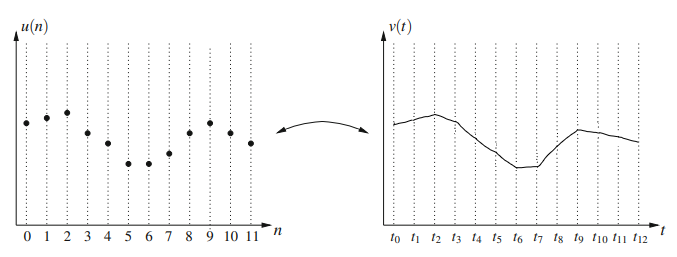
\includegraphics[width=\linewidth]{pics/FOH.png}
	\caption{Illustration of first-order hold}
	\label{fig:FOH}
\end{figure}


\subsection{Runge-Kutta method}
Given a continuous time LTI system in Eq. (\ref{eq:ode}), the corresponding RK discretization models can be represented by the following equation:
\begin{equation}
	x_{k+1} = A_{\rm{rk}}x_k + B_{\rm{rk}}u_k,
	\label{eq5}
\end{equation}

The family of explicit RK methods is given by
\begin{equation}
	x_{k+1} = x_k +  \sum_{i=1}^s b_i \kappa_i,
\end{equation}
where
\begin{equation}
	\begin{split}
		%\frac{dx}{dt} &=  f(t, x), \quad x\left(t_{0}\right)=x_{0},\\
		\kappa_1 &= \Delta t f(t_k,x_k,u_k),\\
		\kappa_2 &= \Delta t f(t_k+c_2\Delta t, x_k+\Delta t(a_{21}\kappa_1),u_k),\\
		\kappa_3 &= \Delta t f(t_k+c_3\Delta t, x_k+\Delta t(a_{31}\kappa_1+a_{32}\kappa_2),u_k)\\
		\vdots\\
		\kappa_s &= \Delta t f(t_k+c_s\Delta t,\\&  \quad x_k+\Delta t(a_{s1}\kappa_1+a_{s2}\kappa_2+\cdots+a_{s,s-1}\kappa_{s-1}),u_k).
	\end{split}
\end{equation}
\\
To specify a particular method, one needs to provide the integer $s$ (the number of stages), and the coefficients $a_{ij}$ (for $1 \leq j <i \leq s$) and $c_i$ (for $i=2,3,\cdots,s$). The matrix consisting of the elements $a_{ij}$, which is called Runge-Kutta matrix, while the $b_i$ and $c_i$ are known as the weights and nodes. More compactly, these parameters are written as so-called Butcher tableaus\cite{grune2017nonlinear} of the form
\begin{table}[H]
  \begin{center}
  	\begin{tabular}{c|l}
  	$c_1$ &  \\
  	$c_2$ & $a_{21}$ \\
  	$c_3$ & $a_{31}$ $a_{32}$\\
  	$\vdots$ & $\vdots$ $\quad$ $\quad$ $\ddots$\\
  	$c_s$ & $a_{s1}$ $a_{s2}$ $\cdots$ $a_{s,s-1}$\\
  	\hline
  	$\quad$ & $b_1\ \ $ $b_2\ $ $\cdots$ $b_{s-1}\ \ $ $b_s$
  	\end{tabular}	
  \end{center}
\end{table}
Table 1 shows Butcher tableaus corresponding to the Euler scheme known as RK1 (left), the Heun scheme known as RK2 (middle) and the so-called classical Runge–Kutta scheme with s = 4 stages proposed by Carl Runge and Martin Kutta in 1895 (right).
\begin{table}[!htb]
	\begin{minipage}{.33\linewidth}
		\caption{}
		\centering
		\begin{tabular}{c|l}
			$0$ &  \\
			\hline
			& 1
		\end{tabular}
	\end{minipage}%
	\begin{minipage}{.33\linewidth}
		\centering
		\caption{}
		\begin{tabular}{c|l}
			$0$ &  \\
			1 & 1  \\
			\hline
			& $\frac{1}{2}$ $\frac{1}{2}$
		\end{tabular}
	\end{minipage} %
    \begin{minipage}{.33\linewidth}
    	\caption{}
    	\centering
    	\begin{tabular}{c|l}
    		$0$ &  \\
    		$\frac{1}{2}$ & $\frac{1}{2}$ \\
    		$\frac{1}{2}$ & $0$ $\frac{1}{2}$\\
    		$1$ & $0$ $0$ $1$            \\
    		\hline
    		& $\frac{1}{6}$ $\frac{2}{6}$ $\frac{2}{6}$ $\frac{1}{6}$
    	\end{tabular}
    \end{minipage}
\end{table}

We solve the MPC problem using numerical optimization methods, therefore the continuous-time dynamical system equations need to be discretized. If control input $u$ is known continuously, then we can directly evaluate $u(t)$ at the given sampling interval of RK method. For example, when using the fourth order Runge-Kutta method with ZOH, using $x_n = x(t_0+n\Delta t)$ and $u_n = u(t_0+n\Delta t)$, then we obtain
\begin{equation}
	\begin{split}
		x_{k+1} &= x_k + \frac{1}{6}(\kappa_1 + 2\kappa_2 +2\kappa_3 + \kappa_4),\\
		\kappa_1 &= \Delta t(A_{\rm{con}}x_k+B_{\rm{con}}u_k),\\
		\kappa_2 &= \Delta t(A_{\rm{con}}(x_k+\kappa_1/2)+B_{\rm{con}}u_k),\\
		\kappa_3 &= \Delta t(A_{\rm{con}}(x_k+\kappa_2/2)+B_{\rm{con}}u_k),\\
		\kappa_4 &= \Delta t(A_{\rm{con}}(x_k+\kappa_3)+B_{\rm{con}}u_k).\\
	\end{split}
\end{equation}
Substituting these equations into each other gives
\begin{equation}
	\begin{split}
	    x_{k+1} &= \underbrace{\left(I + \Delta t A_{\rm{con}} + \frac{{\Delta t}^2}{2!}A_{\rm{con}}^2 + \frac{{\Delta t}^3}{3!}A_{\rm{con}}^3 + \frac{{\Delta t}^4}{4!}A_{\rm{con}}^4\right)}_{\rm{A_{rk4}}}x_k\\
	    &+ \underbrace{\left(\Delta t I  + \frac{{\Delta t}^2}{2!}A_{\rm{con}} + \frac{{\Delta t}^3}{3!}A_{\rm{con}}^2 + \frac{{\Delta t}^4}{4!}A_{\rm{con}}^3\right)B_{\rm{con}}}_{\rm{B_{rk4}}}u_k.
	\end{split}
\end{equation}
Therefore, the system matrices $A_{\rm{rk}}$ and $B_{\rm{rk}}$ in (5) are:
\begin{equation}
	\begin{split}
		A_{\rm{rk4}} &= I + \Delta t A_{\rm{con}} + \frac{{\Delta t}^2}{2!}A_{\rm{con}}^2 + \frac{{\Delta t}^3}{3!}A_{\rm{con}}^3 + \frac{{\Delta t}^4}{4!}A_{\rm{con}}^4,\\
		B_{\rm{rk4}} &= \left(\Delta t I  + \frac{{\Delta t}^2}{2!}A_{\rm{con}} + \frac{{\Delta t}^3}{3!}A_{\rm{con}}^2 + \frac{{\Delta t}^4}{4!}A_{\rm{con}}^3\right)B_{\rm{con}}.
	\end{split}
\end{equation}
Similar to RK4 approximation, we can obtain the system matrices of RK1 and RK2 methods:
\begin{equation}
	\begin{split}
		A_{\rm{rk1}} &= I + \Delta t A_{\rm{con}},\\
		B_{\rm{rk1}} &= \Delta tB_{\rm{con}},\\
		A_{\rm{rk2}} &= I + \Delta t A_{\rm{con}} + \frac{{\Delta t}^2}{2!}A_{\rm{con}}^2,\\
		B_{\rm{rk2}} &= \left(\Delta t I  + \frac{{\Delta t}^2}{2!}A_{\rm{con}}\right)B_{\rm{con}}.
	\end{split}
\end{equation}

\subsection{Gauss collocation method}
Using $s$-stage Gauss collocation, we can get the numerical approximation of the discrete-time model. 
The Gauss collocation numerical solution with state stage values $x_{k}^{o, i}$, $i = 1,...,s$:
\begin{equation}
	\begin{split}
		{x}_{k+1} &={x}_{k}+ \Delta t \sum_{i=1}^{s} b_{i}^{s} \mathbf{f}\left(\mathbf{x}_{k}^{o, i}\right)+\Delta t \mathbf{g} \sum_{i=1}^{s} b_{i}^{s} u_{k}^{i} ,\\ {x}_{k}^{o, i} &={x}_{k}+\Delta t \sum_{j=1}^{s} a_{i j}^{s} \mathbf{f}\left(\mathbf{x}_{k}^{o, j}\right)+\Delta t \mathbf{g} \sum_{j=1}^{s} a_{i j}^{s} u_{k}^{j} ,
	\end{split}
\end{equation}
where the RK coefficients $a_{i j}^{s} =\int_{0}^{c_{j}} \ell_{i}^{s-1}(\tau) d \tau$ and $b_{i}^{s} =\int_{0}^{1} \ell_{i}^{s-1}(\tau) d \tau$.
In Gauss collocation method, the control input $u_k$ can be shaped with Lagrange polynomials. The control input for $t \in\left[t_{k}, t_{k+1}\right)$ generated via an $s-1$ order hold element using Lagrange interpolation polynomials \cite{kotyczka2021high}:
\begin{equation}
	u\left(t_{k}+\tau \Delta t\right)=\sum_{i=1}^{s} u_{k}^{i} \ell_{i}^{s-1}(\tau),
\end{equation}
where $$
\ell_{i}^{s-1}(\tau)=\prod_{\substack{l=1 \\ l \neq i}} \frac{\tau-c_{l}}{c_{i}-c_{l}}.
$$
The control stage values in the collocation points (weights of Lagrange polynomials):
$$
u\left(t_{k}^{i}\right)=u_{k}^{i}, \quad t_{k}^{i}=t_{k}+c_{i} \Delta t, \quad i=1, \ldots, s
$$
The collocation points on the unit interval are shown in Fig.~\ref{fig:gausscoll}, the collocation points $c_{1}^{0}=\frac{1}{2}$ and $c_{1 / 2}^{1}=\frac{1}{2} \mp \frac{\sqrt{3}}{6}$
\begin{figure}[h]
	\centering
	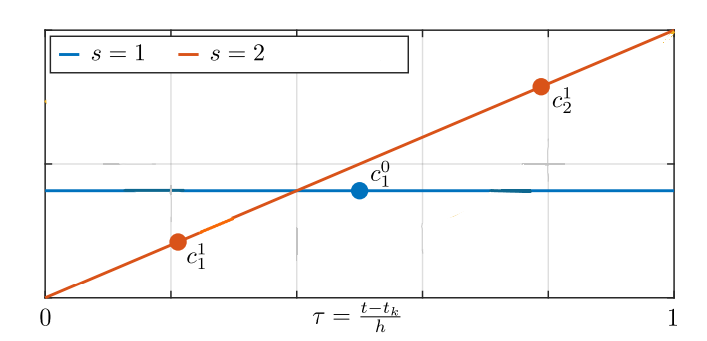
\includegraphics[width=\linewidth]{pics/gausscoll.png}
	\caption{Control signal shapes on the unit interval based on Gauss collocation points}
	\label{fig:gausscoll}
\end{figure}
\\\\
Given the same continuous time LTI system in (\ref{eq:ode}), the corresponding Gauss collocation discretization models can be represented by an equation of the form (4).
\subsubsection{Zero-order hold control input}
When $s = 1$, i.e. the zero-order hold case, the control input for $t \in \left[t_k, t_{k+1}\right]$ results in
$$u(t) = u_k$$
\\
The exact discretization model can be represented as:
\begin{equation}
	x_{k+1} = A_{\rm{ex,1}}x_k+B_{\rm{ex,1}}u_k,
\end{equation}
where $A_{\rm{ex,1}} = e^{A_{\rm{con}}  \Delta t}$ and $B_{\rm{ex,1}} = \int_{0}^{\Delta t} e^{A_{\rm{con}}  \tau}  B_{\rm{con}} d \tau$.
\\\\
Using (12), the Gauss collocation numerical discretization of order s = 1 yields
\begin{equation}
	\begin{split}
		x_{k+1}&=x_{k}+\Delta t  b_{1}  A_{\rm{con}}  x_{k}^{1}+\Delta t  b_{1}  B_{\rm{con}}  u_{k}^{1},\\
		x_{k}^{1}&=x_{k}+\Delta t a_{11} A_{\rm{con}} x_{k}^{1}+\Delta t  a_{11} B_{\rm{con}} u_{k}^{1}.
	\end{split}
\label{zerocoll}
\end{equation}
We can reformulate (\ref{zerocoll}) into the explicit LTI form (4)
with
$$
A_{\rm{d}} = I+\Delta t  b_1  A_{\rm{con}}  (I-\Delta t  a_{11}  A_{\rm{con}})^{-1},
$$
$$
B_{\rm{d}} = \Delta t  b_1  A_{\rm{con}}  (I-\Delta t  a_{11}  A_{\rm{con}})^{-1}  \Delta t  a_{11}  B_{\rm{con}} + \Delta t  b_1  B_{\rm{con}}.
$$
Note that all the used inverse matrices have to exist, otherwise, the derivation is not possible.

\subsubsection{First-order hold control input}
When $s = 2$, i.e. the first-order hold case, the control input for $t \in \left[t_k, t_{k+1}\right]$ results in
\begin{equation}
	\begin{split}
        u(t) &= u_k^{1}  l^1(t)+u_k^2  l^2(t)\\
        &= u_k^{1}  \frac{t-c_2^1}{c_1^1-c_2^1} +u_k^2 \frac{t-c_1^1}{c_2^1-c_1^1}.
    \end{split}
\end{equation}
Note that in the case of FOH input, not only the Gauss collocation points should satisfy the input constraints, but also the starting and ending points of the piecewise linear function.
\\
The exact discretization model can be represented as:
\begin{equation}
    x_{k+1} = A_{\rm{ex,2}}x_k+B_{\rm{ex,2}}\begin{bmatrix}
    	u_{k}^1 \\
    	u_{k}^{2}
    \end{bmatrix}
\end{equation}
with
$$
A_{\rm{ex,2}} = e^{A_{\rm{con}}  \Delta t},
$$
$$
B_{\rm{ex,2}} = \int_{0}^{\Delta t} e^{A_{\rm{con}} \tau}  B_{\rm{con}}  \begin{bmatrix}
	l^1\left(\frac{\Delta t - \tau}{\Delta t}\right),      & l^2\left(\frac{\Delta t - \tau}{\Delta t}\right) 
\end{bmatrix}  d \tau.
$$
\\
The Gauss collocation numerical discretization model can be represented as:
\begin{equation}
	\begin{split}
		x_{k+1}&=x_{k}+\Delta t  b_{1}  A_{\rm{con}}  x_{k}^{1}+\Delta t  b_{2}  A_{\rm{con}}  x_{k}^{2} \\ & \quad+\Delta t  b_{1}  B_{\rm{con}}  u_{k}^{1}+\Delta t  b_{2}  B_{\rm{con}}  u_{k}^{2}, \\
		x_{k}^{1}&=x_{k}+\Delta t  a_{11}  A_{\rm{con}}  x_{k}^{1}+\Delta t  a_{12}  A_{\rm{con}}  x_{k}^{2} \\ & \quad +\Delta t  a_{11}  B_{\rm{con}}  u_{k}^{1}+\Delta t  a_{12}  B_{\rm{con}}  u_{k}^{2}, \\
		x_{k}^{2}&=x_{k}+\Delta t  a_{21}  A_{\rm{con}}  x_{k}^{1}+\Delta t  a_{22}  A_{\rm{con}}  x_{k}^{2} \\ & \quad +\Delta t  a_{21}  B_{\rm{con}}  u_{k}^{1}+\Delta t  a_{22}  B_{\rm{con}} u_{k}^{2}.
	\end{split}
	\label{firstcoll}
\end{equation}
We can reformulate (\ref{firstcoll}) into the explicit LTI form (4)
with
\begin{equation}
	\begin{split}
    	A_{\rm{d}}&=I+A_{b1}  A_{\rm{1inv}}  \left( I+ A_{a12} \left(I-A_{a22}\right)^{-1} \right) \\ & \quad+A_{b2}  A_{\rm{2inv}}  \left(I+A_{a21} \left(I-A_{a11}\right)^{-1}\right),\\
    	A_{\rm{1i n v}}&=\left(  I-A_{a11}-A_{a12}  \left(I-A_{a22}\right)^{-1}  A_{a21}\right)^{-1},\\
    	A_{\rm{2 i n v}} &=\left(I-A_{a21} \left(I-A_{a11}\right)^{-1}  A_{a12}-A_{a22}\right)^{-1},
	\end{split}
\end{equation}

\begin{equation}
	\begin{split} 
		B_{\rm{d}}=&\left[A_{b 1}  A_{\rm{1inv}} \left(A_{a 12} \left(I-A_{a 22}\right)^{-1}  B_{a 21}+B_{a 11}\right)+\right. \\
		&A_{b 2}  A_{\rm{2 i n v}} \left(A_{a 21} \left(I-A_{a 11}\right)^{-1}  B_{a 11}+B_{a 21}\right)+B_{b 1} ,\\
		&A_{b1}  A_{\rm{1inv}} \left(A_{a 12} \left(I-A_{a_{22}}\right)^{-1}  B_{a_{22}}+B_{a 12}\right)+\left. \right.\\
		&\left.A_{b 2}  A_{\rm{2 i n v}} \left(A_{a_{21}} \left(I-A_{a 11}\right)^{-1}  B_{a 12}+B_{a 22}\right)+B_{b 2}\right],
	\end{split}
\end{equation}
and
\begin{equation}
	\begin{split}
        A_{a i j} &=\Delta t  a_{i j}  A_{\rm{c o n}}, \\
        B_{a i j} &=\Delta t  a_{i j}  B_{\rm{c o n}}, \\
        A_{b i} &=\Delta t  b_{i}  A_{\rm{c o n}}, \\
        B_{b i} &=\Delta t  b_{i}  B_{\rm{c o n}}. \\
	\end{split}
\end{equation}
Note that all the used inverse matrices have to exist, otherwise, the derivation is not possible.
\section{Implementation and Evaluation}
In the following, we will implement an example to compare the different-order hold RK methods and Gauss collocation method. For the RK methods, we will firstly compare the discretization accuracy of the state trajectory of the true continuous system using different RK methods, then we investigate the control invariant set and classic variant set of different RK methods. For the Gauss collocation method, we will compare the exact discretization model and the corresponding Gauss collocation model that consider piecewise polynomial input functions.
\subsection{Runge-Kutta method}
The RK discretization models can be structured by the matrices $A_{rk}$ and $B_{rk}$ and apply them to (\ref{eq5}) , we will assume a piecewise constant control ZOH, so we can focus on how the state trajectory discretization is handled. We will consider three discretization models, which are RK1, RK2 and RK4 models.
First, we will be driving a continuous time LTI system to the origin. We will minimize a quadratic cost, so we define the cost terms $l_k$ and $l_N$
\begin{equation}
	\begin{split}
		l_k &= x_k^TQx_k + u_k^TRu_k\\
		l_N &= x_{k+N}^TQ_Nx_{k+N}
	\end{split}
\end{equation}
where the matrices $Q \in \mathbb{R}^{m \times m}$, $R \in \mathbb{R}^{n \times n}$ and $Q_N \in \mathbb{R}^{m \times m}$ are symmetric definite positive.
The continuous time system is given by the system matrices
\begin{equation}
	\begin{split}
		A_{\text {con }}=\left[\begin{array}{cc}
			0 & 7.5 \\
			-1.5 & -0.1
		\end{array}\right], \quad B_{\text {con }}=\left[\begin{array}{c}
			0.145 \\
			0.5
		\end{array}\right].
	\end{split}
\end{equation}
The initial condition is $x(0) = [2,2]^{\top}$ and the state and control input is subject to the following constraints
\begin{equation}
	\begin{split}
		 -1 \leq\  &x_1 \leq 2.8\\
		 -1 \leq\  &x_2 \leq 2.1\\
		 -26 \le\  &  u \le 26\\
	\end{split}
\end{equation}
The following steps investigate the closed-loop performance:
\begin{enumerate}
	\item Given the continuous time system, apply different discretization methods (RK of different order, and also vary the sampling time/discretization grid) to retrieve different discretized models.
	
	\item Apply an MPC iteration to retrieve an optimal (discrete time) control input. This control input is then applied to the true continuous system in a ZOH fashion, thus, constantly apply the retrieved optimal control input for the duration of one sampling time of the current discrete system. We will then retrieve the new current state.
\end{enumerate}
The chosen sampling time is $\Delta t = 0.04$ seconds, the horizon length is N = 10, and the weight matrix are $Q = Q_N =$diag$([10,1])$ and R = 1.
The state trajectory of the true continuous system is shown in Fig. \ref{fig:statetrajec0.04}
\begin{figure}[h!]
	\centering
	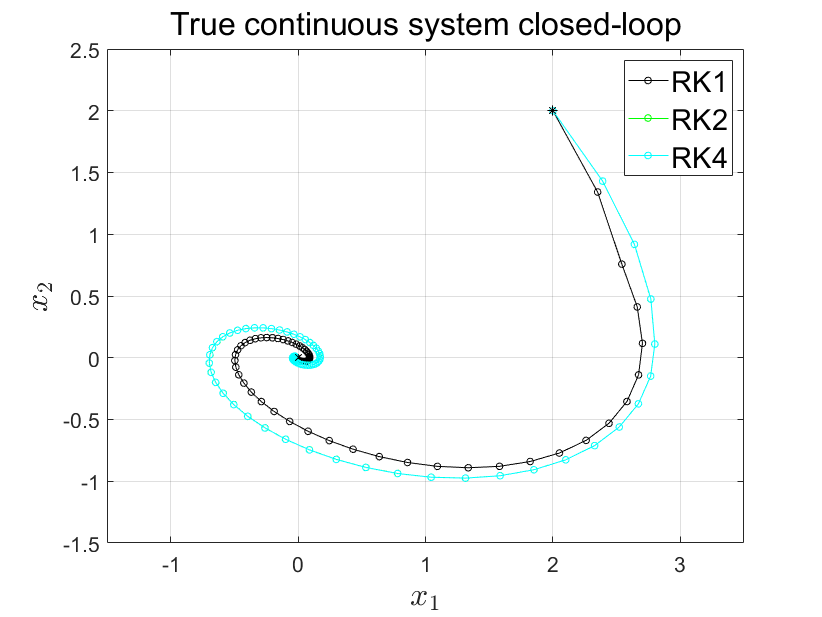
\includegraphics[width=\linewidth]{pics/deltat = 0.04.png}
	\caption{State trajectory of true continuous system}
	\label{fig:statetrajec0.04}
\end{figure}
\newline
In Fig. \ref{fig:statetrajec0.04}, the black line represents the system behavior of RK1 model, while the RK2 has a green line, and it coincides with the cyan line in the plot, which means that the approximation performance between RK2 and RK4 models at a sampling time of $0.04$ seconds is extremely similar.
Now assume that the sampling time $\Delta t = 0.02$ seconds, the corresponding state trajectory of the true system is shown in Fig. \ref{fig:statetrajec0.02}.
\begin{figure}[H]
 	\centering
 	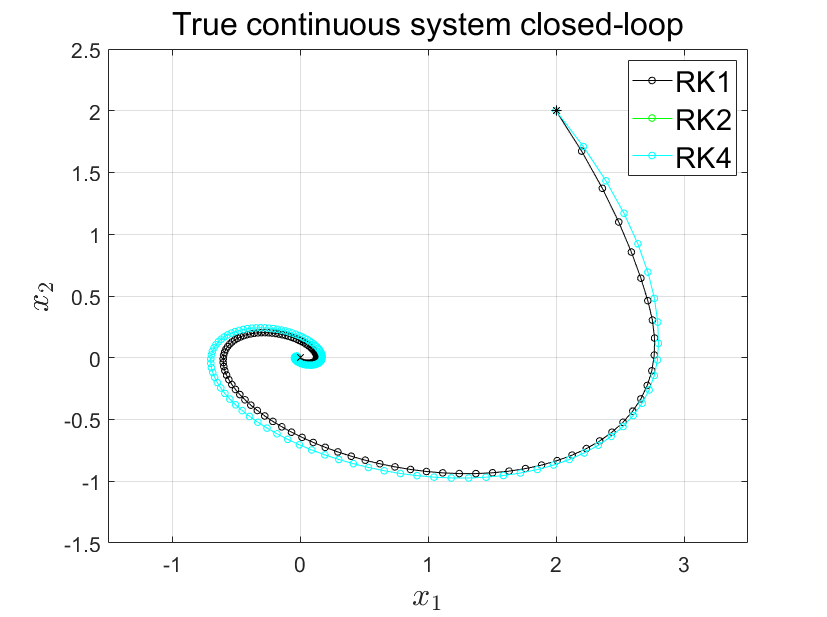
\includegraphics[width=\linewidth]{pics/deltat = 0.02.png}
 	\caption{State trajectory of true continuous system}
 	\label{fig:statetrajec0.02}
\end{figure}

In Fig. \ref{fig:statetrajec0.02}, it can be observed that the black line of RK1 is closer to the green line with a smaller sampling time $\Delta t$, which indicates that the shorter sampling time, the higher the accuracy.
\newline
In Fig. \ref{fig:statetrajec0.020.04}, we apply a smaller sampling time $\Delta t = 0.008$ for RK1 model, while applying a larger sampling time $\Delta t = 0.04$ for RK2 and RK4 models, the state trajectory of three models are extremely similar, which indicates decreasing the sampling time $\Delta t$ of RK1 model so that it has the same accuracy as RK2 and RK4 models with larger sampling time $\Delta t$.
 \begin{figure}[h!]
	\centering
	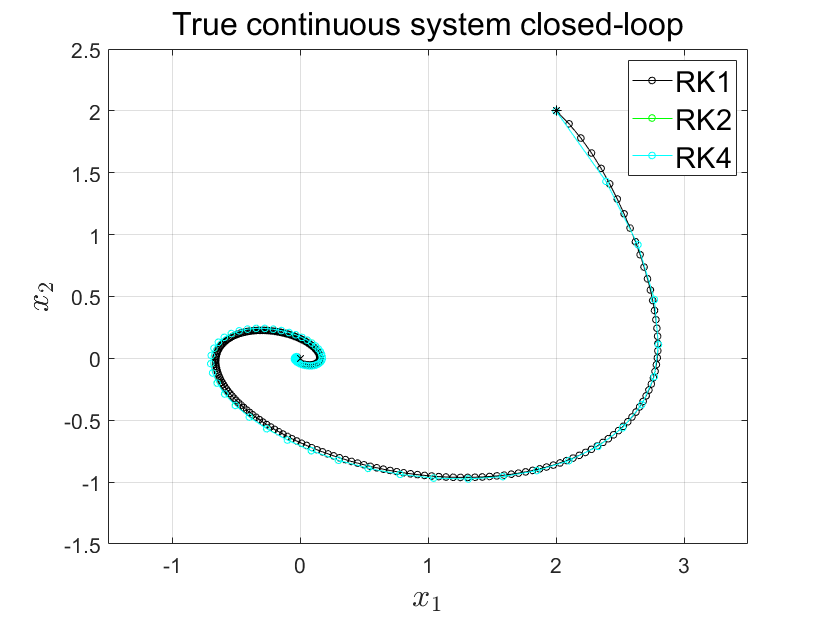
\includegraphics[width=\linewidth]{pics/delta0.04rk10.02rk2rk4.png}
	\caption{State trajectory of true continuous system}
	\label{fig:statetrajec0.020.04}
\end{figure}
\newline
\\
We can achieve similar accuracy between RK1 model with small sampling time and RK4 model with large sampling time, however, this yields increased computational cost due to the increased number of optimization steps. Fig. \ref{fig:timempc} shows the time consumption for RK1 model with sampling time $\Delta t = 0.008$ and RK4 model with sampling time $\Delta t =0.04$ of each MPC iteration.
\begin{figure}[H]
	\centering
	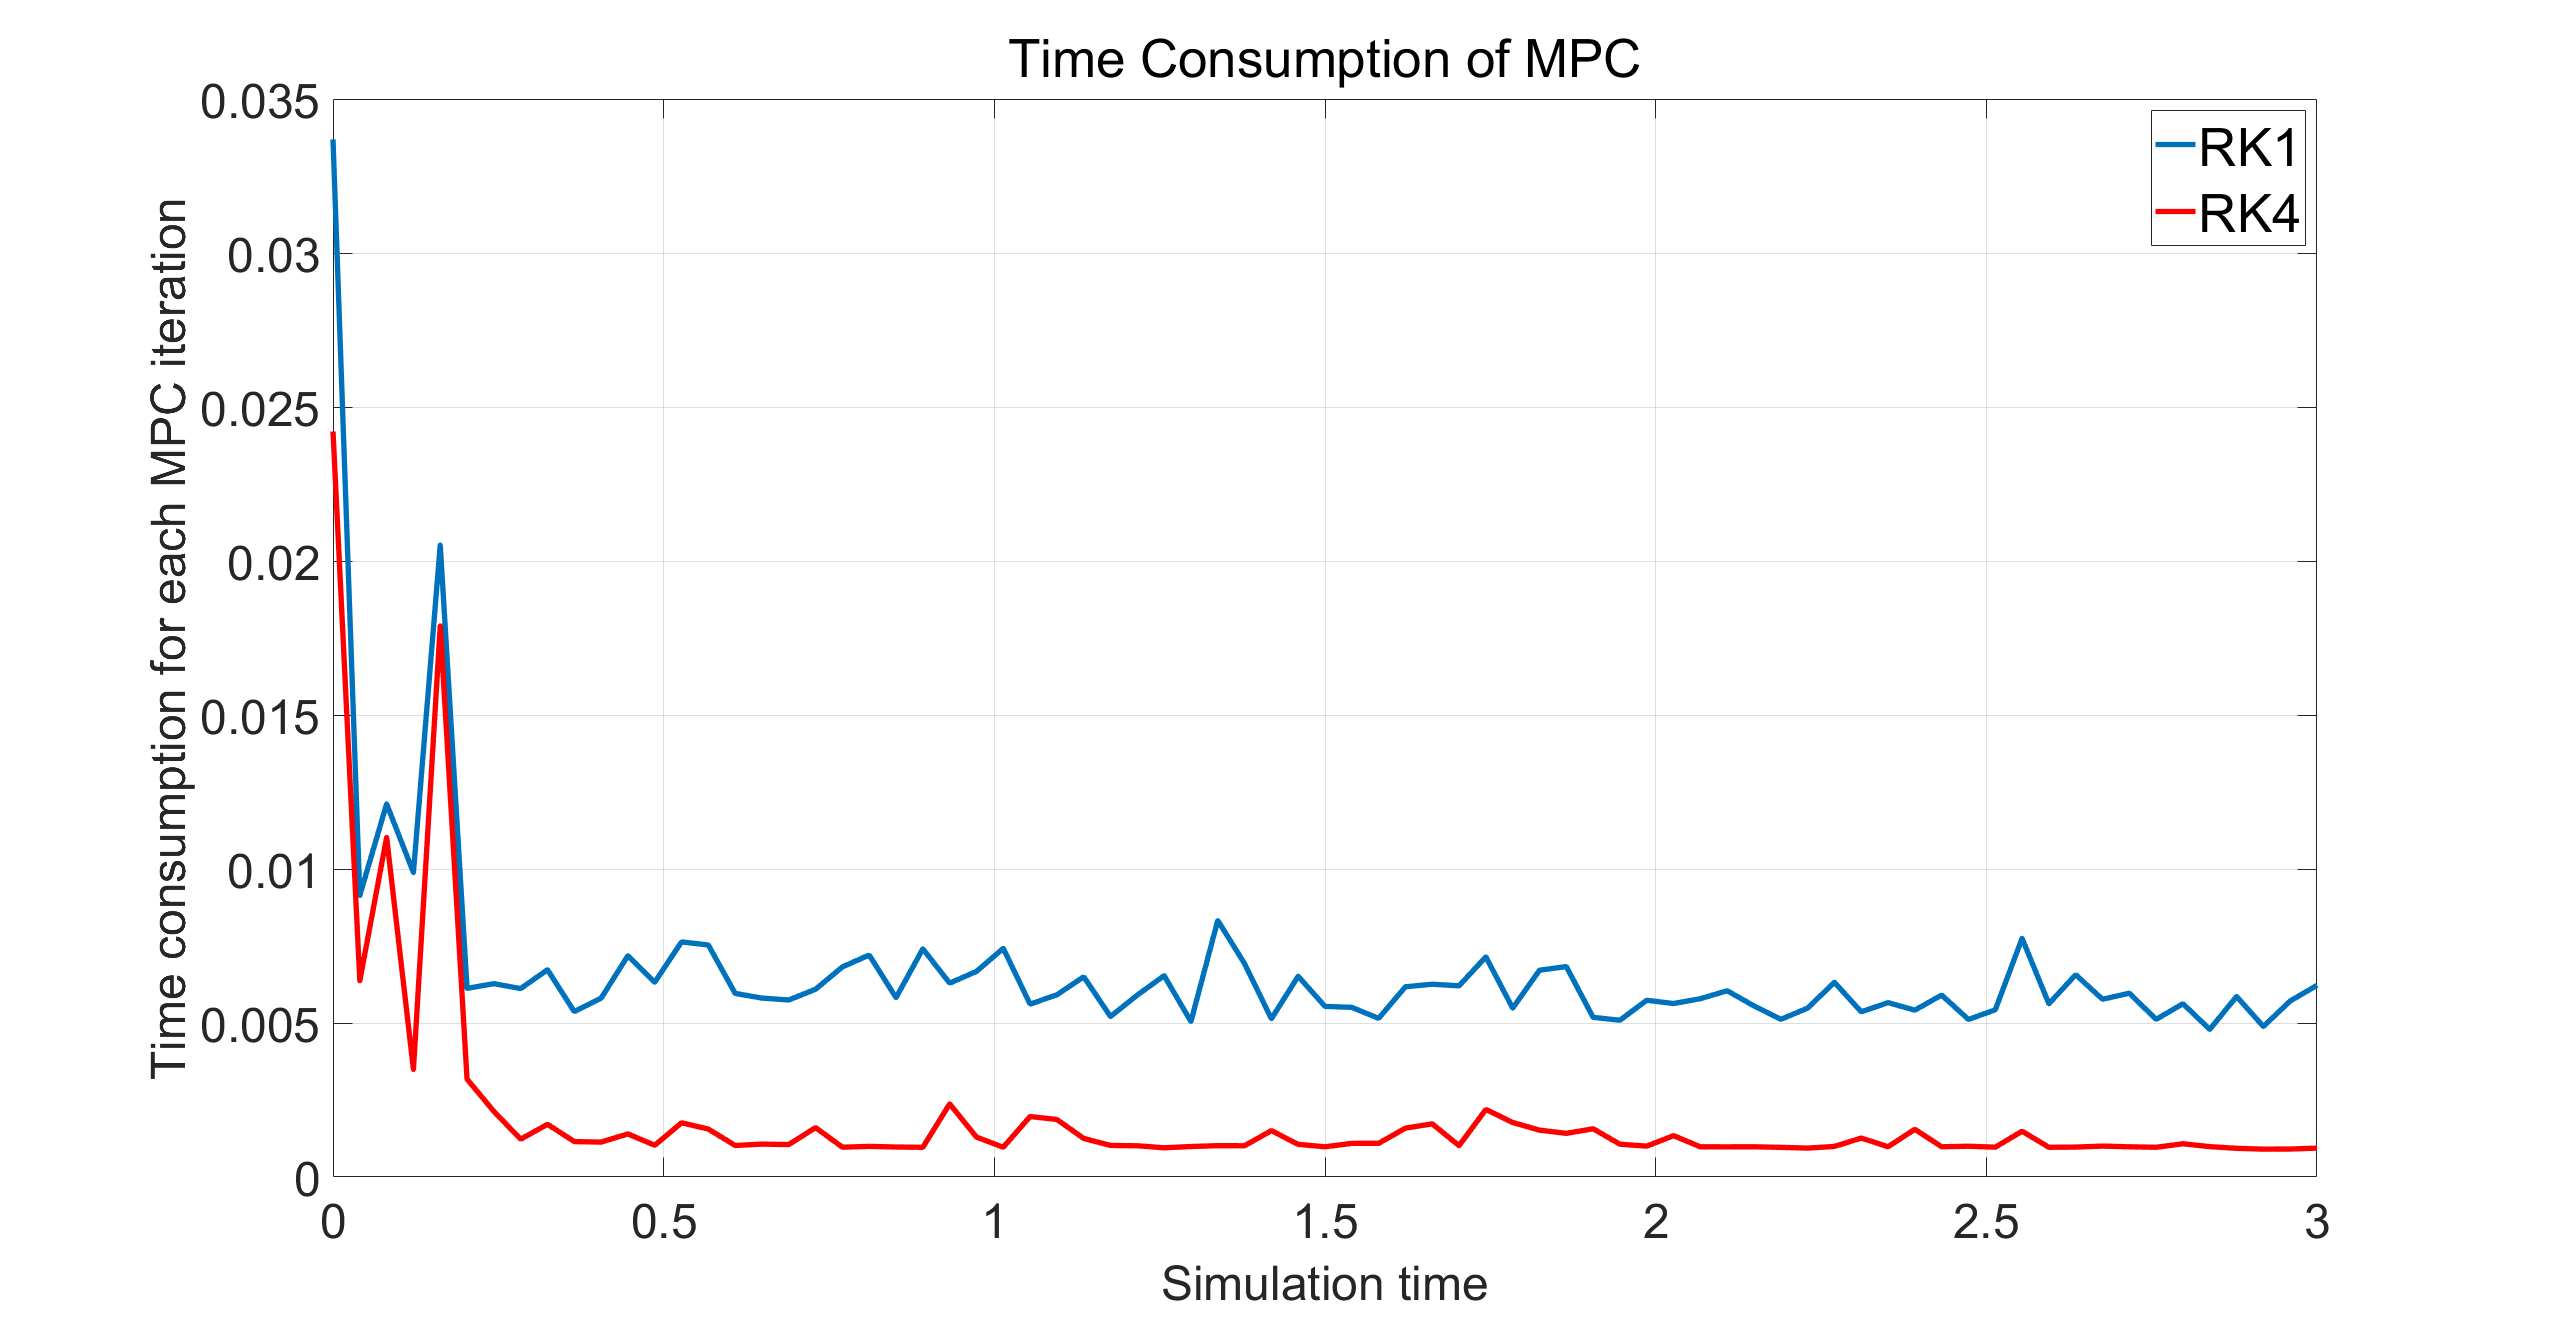
\includegraphics[width=\linewidth]{pics/timempc.png}
	\caption{Time consumption of MPC iteration}
	\label{fig:timempc}
\end{figure}
It is clear that there is a peak in computation time in the first few MPC iterations, which is due to the fact that state $x_1$ here violates the constraint and takes longer to compute the optimal control input $u$.

Next step, we investigates the open-loop performance:
\begin{enumerate}
	\item  Given the continuous time system, apply different discretization methods (RK of different order, and also vary the sampling time/discretization grid) to retrieve different discretized models.
	
	\item Apply an MPC iteration to retrieve an optimal (discrete time) control input sequence.
	
	\item  Apply the control input sequence to the discretized model, and also transform the control input sequence to a continuous time sequence using ZOH and apply it to the true (continuous) system dynamics.
\end{enumerate}
The prediction accuracy of different RK models vary from sampling time, the results shown in Table below
\begin{table}[H]
	\centering
	\begin{tabular}{|c|c|c|c|}
		\hline
		\diagbox{$\Delta$ t}{Error}{RK model}&RK1&RK2&RK4\\ 
		\hline
		0.04&0.323&0.095&0.102\\
		\hline
		0.02&0.081&0.063&0.062\\
		\hline
	\end{tabular}
\end{table}
\begin{equation}
	\epsilon = \frac{\sum_{k=1}^{N} |x_{\rm{con}}(k) - x_{\rm{pre}}(k)|}{N},
\end{equation}
where $N = T/ \Delta t$, $x_{\rm{con}}(k)$ is the true continuous system predicted states at step $k$ and $x_{\rm{pre}}(k)$ is the MPC predicted states at step $k$.

Next, we investigate the control invariant set and the invariant set for the uncontrolled system. Fig. \ref{fig:coninvesetrk1} shows the control invariant set of RK1 and RK4 model with sampling time $\Delta t = 0.06$.
\begin{figure}[H]
	\centering
	\begin{subfigure}[b]{0.37\textwidth}
		\centering
		\includegraphics[width=\linewidth]{pics/coninvset0.06.png}
		\caption{The control invariant set for RK1 model}
		\label{fig:coninvesetrk1}
	\end{subfigure}
	\hfill
	\begin{subfigure}[b]{0.37\textwidth}
		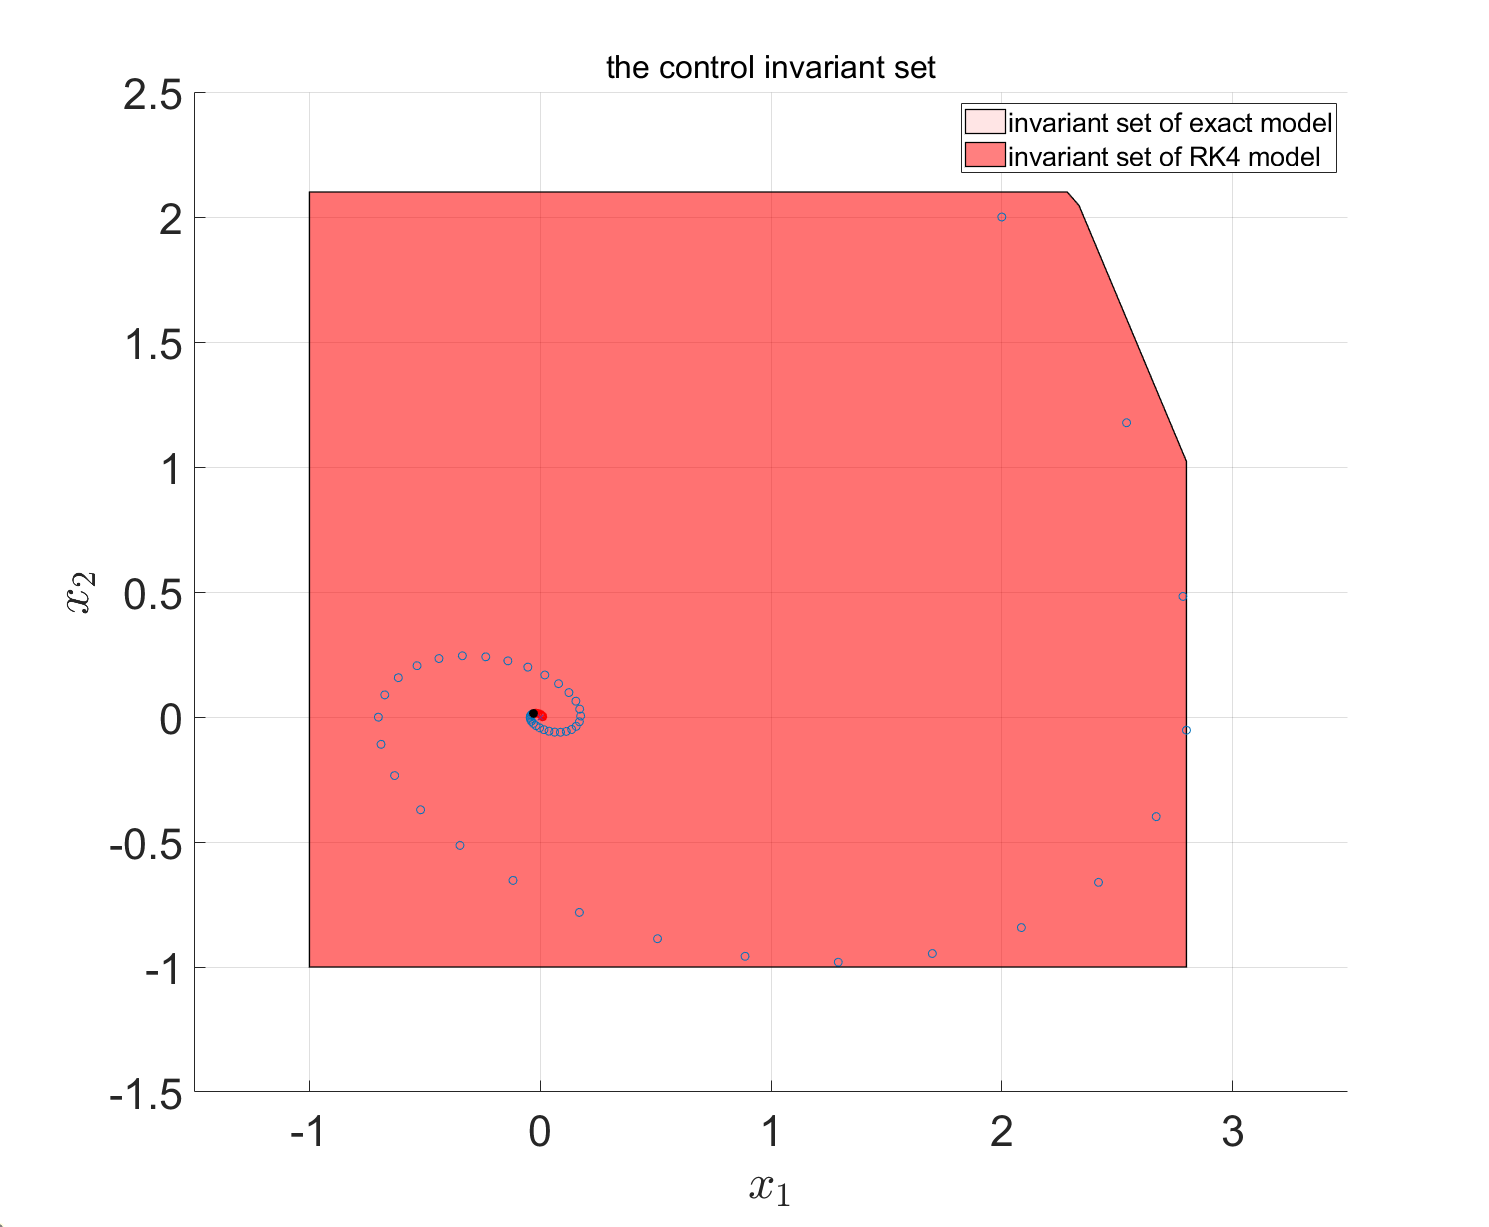
\includegraphics[width=\linewidth]{pics/CONINVSETRK40.06.png}
		\caption{The control invariant set for RK4 model}
		\label{fig:coninvesetrk4}
	\end{subfigure}
    \caption{The control invariant set}
	\label{The control invariant set}
\end{figure}

Compared to the control invariant set of the exact model, the initial state $x_0 = [2,2]^{\top}$ is not in the control invariant set of RK1 model, thus, it is impossible to derive an feasible control input $u$, such that $x_1$ does not violate the state constraint, which indicates the inaccuracy and limitations of the RK1 model.

Fig. \ref{fig:coninvesetrk4} shows the control invariant set of RK4 is the same as the one of exact model, which indicates the higher accuracy compared to RK1 model.

Fig. \ref{fig:invesetrk1} and \ref{fig:invesetrk4} shows the invariant set of RK1 and RK4 model with sampling time $\Delta t = 0.03$.
\begin{figure}[H]
	\centering
	\begin{subfigure}[b]{0.37\textwidth}
		\centering
		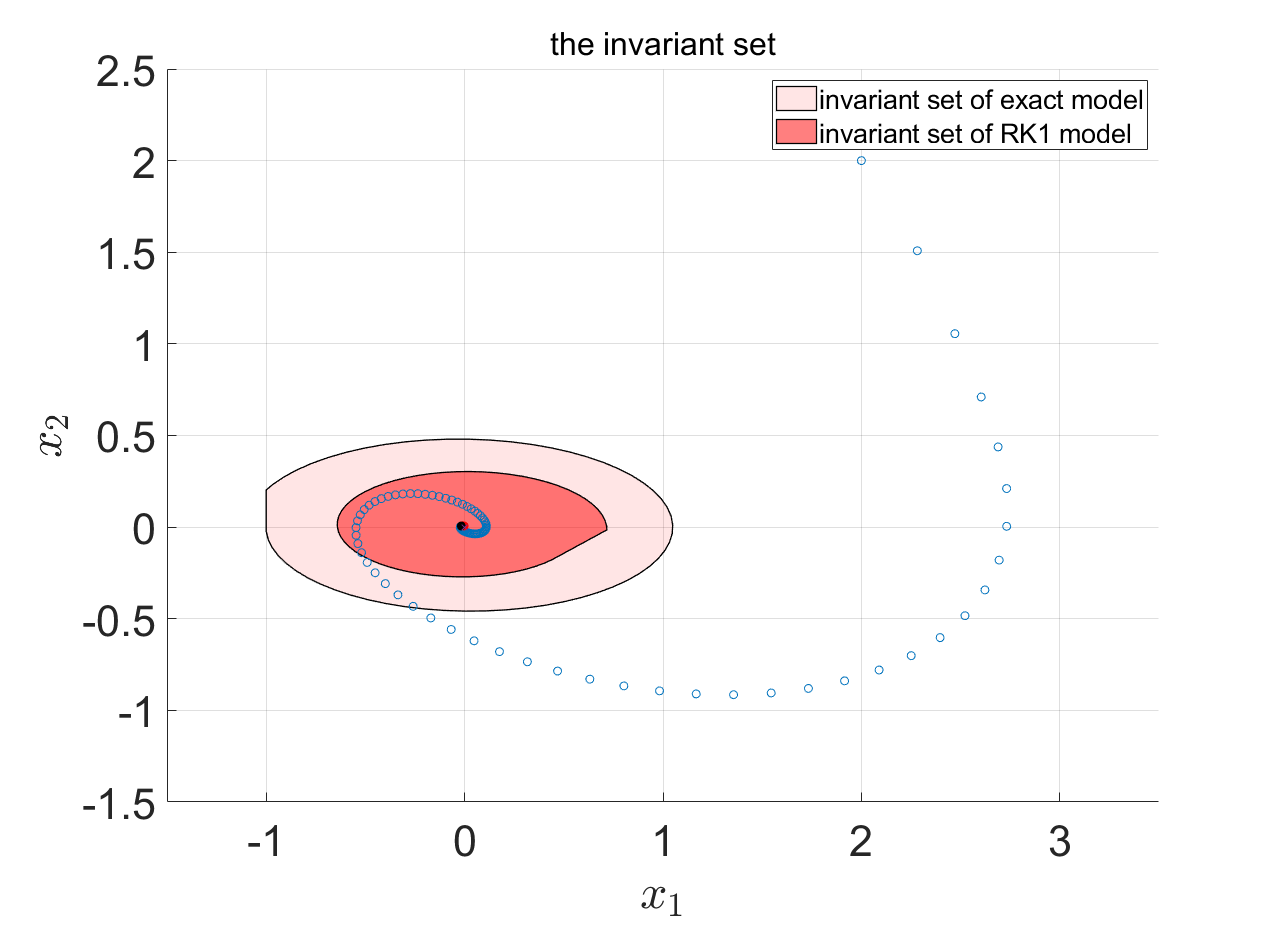
\includegraphics[width=\linewidth]{pics/invsetrk1.png}
		\caption{The invariant set of RK1}
		\label{fig:invesetrk1}
	\end{subfigure}
	\hfill
	\begin{subfigure}[b]{0.37\textwidth}
		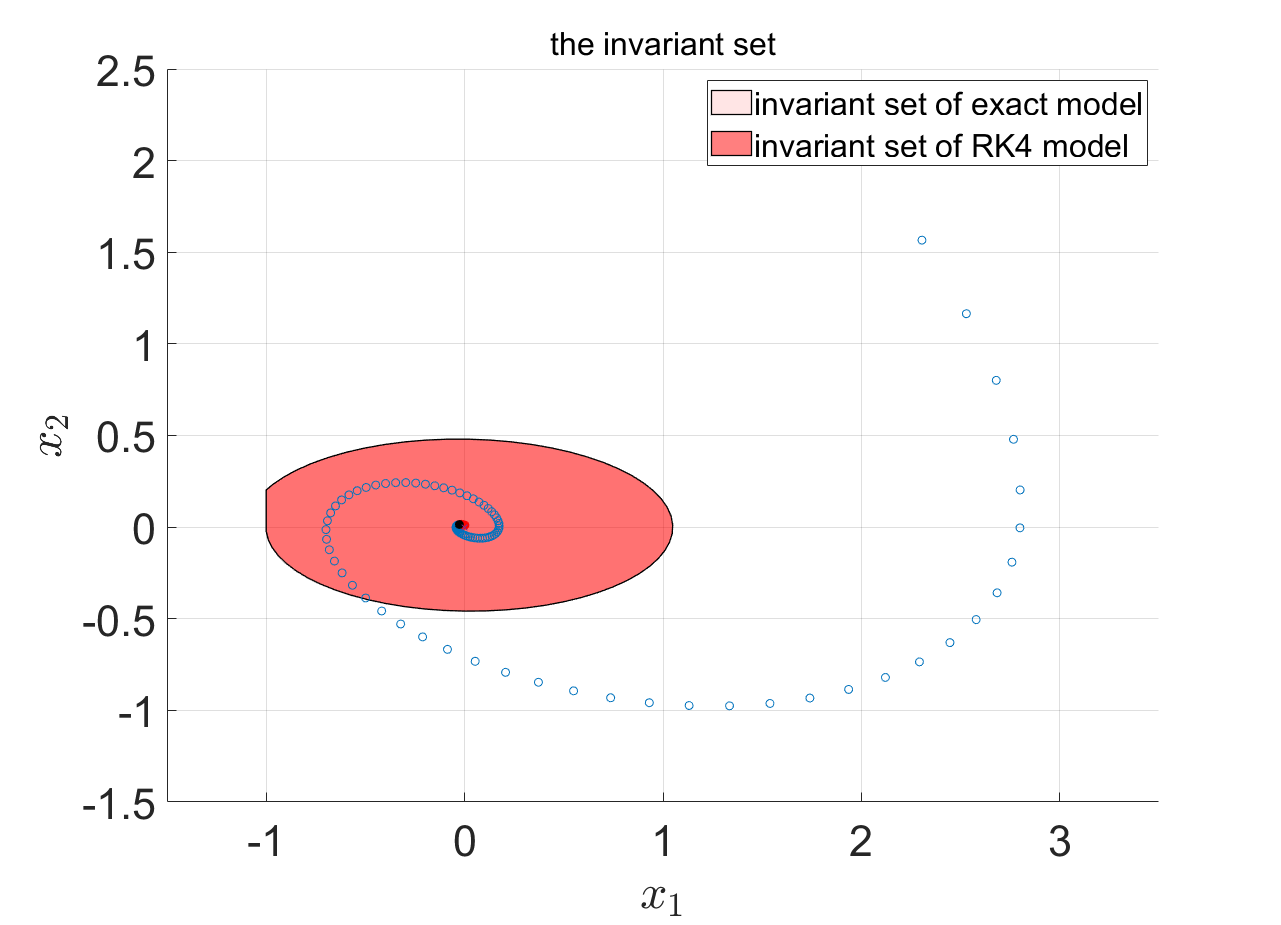
\includegraphics[width=\linewidth]{pics/invsetrk4.png}
		\caption{The invariant set of RK4}
		\label{fig:invesetrk4}
	\end{subfigure}
    \caption{The invariant set}
	\label{fig:The invariant set}
\end{figure}

Similar to the control invariant set, the invariant set for the uncontrolled system of RK1 model is less accurate than the one of RK4 model.
\subsection{Gauss collocation method}
For the Gauss collocation model, the discretized system matrices $A_d$ and $B_d$ are different with different order hold control input $u$. In this example, the ZOH and FOH are implemented. The state trajectory of the Gauss collocation method is compared with the corresponding exact discretized model, whose system matrices are $A_{\rm{ex}}$ and $B_{\rm{ex}}$.

Fig. \ref{fig:gczero.png} shows the state trajectory of exact model and Gauss collocation model with the sampling time $\Delta t = 0.04$ in the case of ZOH. Fig. \ref{fig:ZOHINPUT} shows the corresponding ZOH control input signal.
\begin{figure}[h!]
	\centering
	\begin{subfigure}[b]{0.37\textwidth}
		\centering
		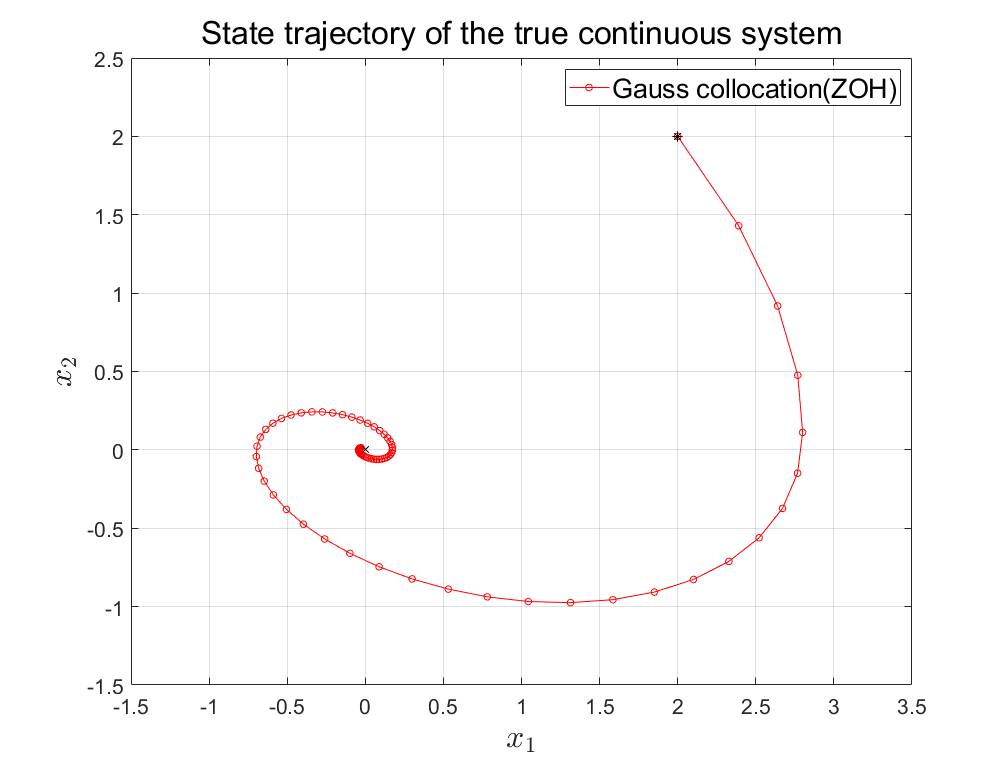
\includegraphics[width=\linewidth]{pics/gczero.png}
		\caption{State trajectory of the true continuous system for ZOH}
		\label{fig:gczero.png}
	\end{subfigure}
	\hfill
	\begin{subfigure}[b]{0.37\textwidth}
		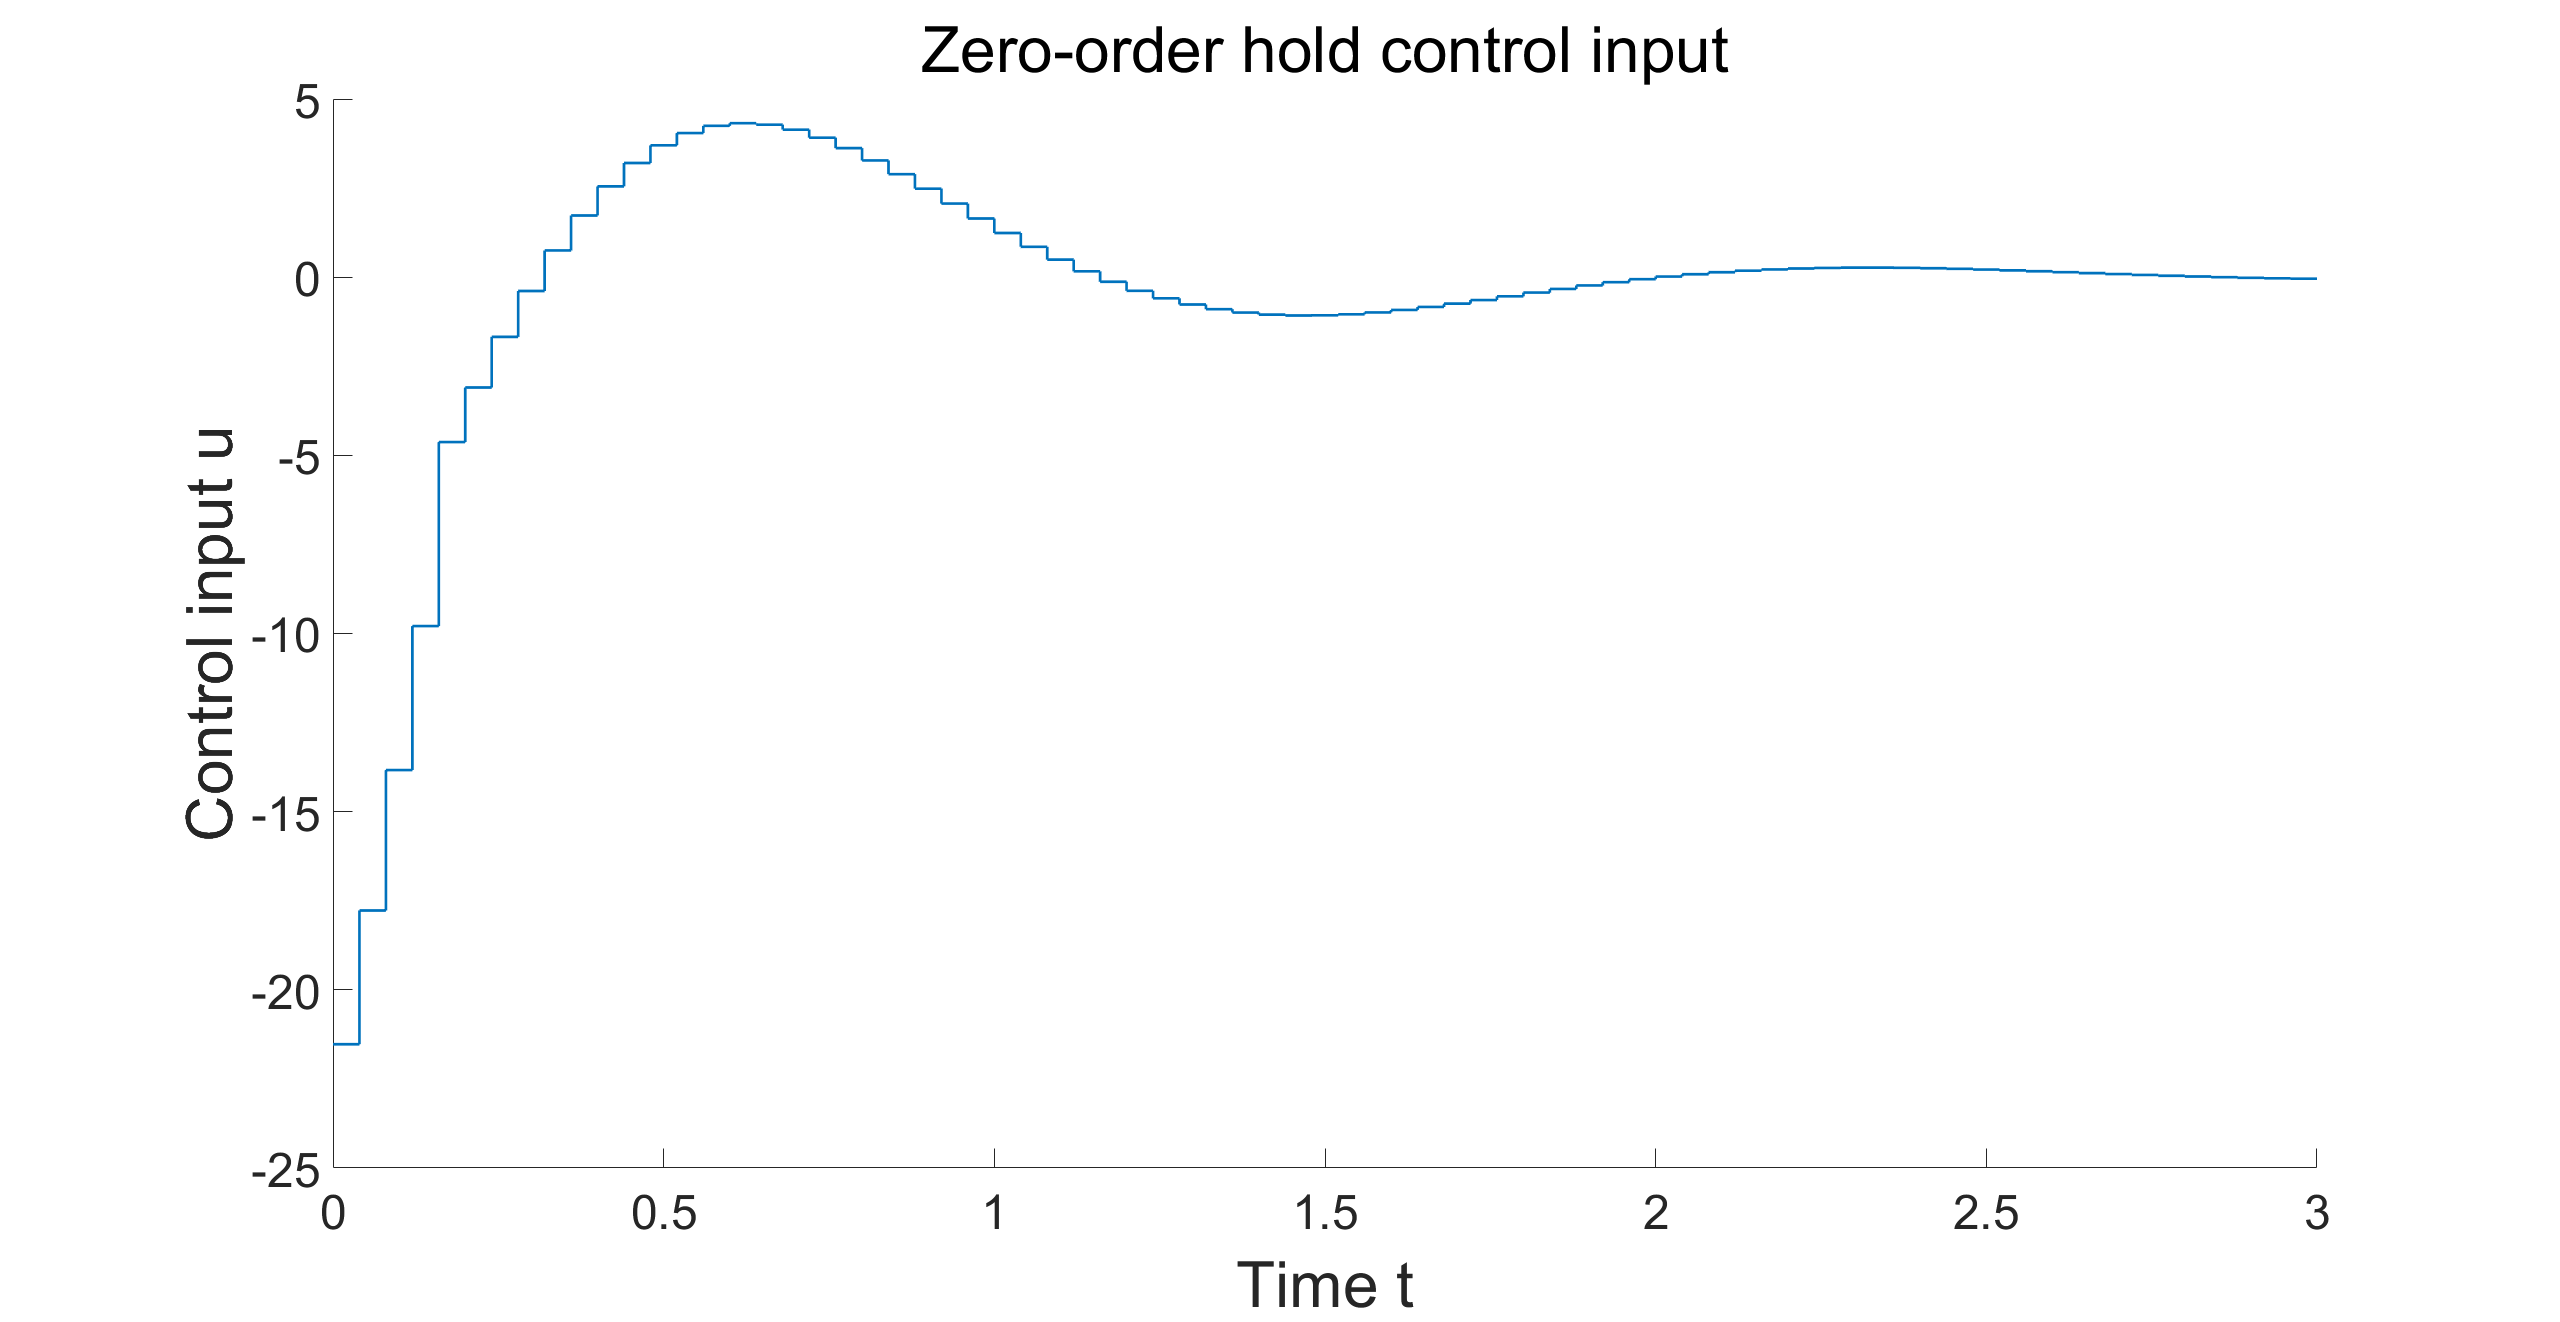
\includegraphics[width=\linewidth]{pics/ZOHINPUT.png}
		\caption{ZOH control input}
		\label{fig:ZOHINPUT}
	\end{subfigure}
	\caption{The state trajectory and ZOH control input}
	\label{fig:The ZOH}
\end{figure}

Fig. \ref{fig:gcfirst.png} shows the state trajectory of exact model and Gauss collocation model with the sampling time $\Delta t = 0.04$ in the case of FOH. Fig. \ref{fig:FOHINPUT} shows the corresponding FOH control input signal.
\begin{figure}[H]
	\centering
	\begin{subfigure}[b]{0.37\textwidth}
		\centering
		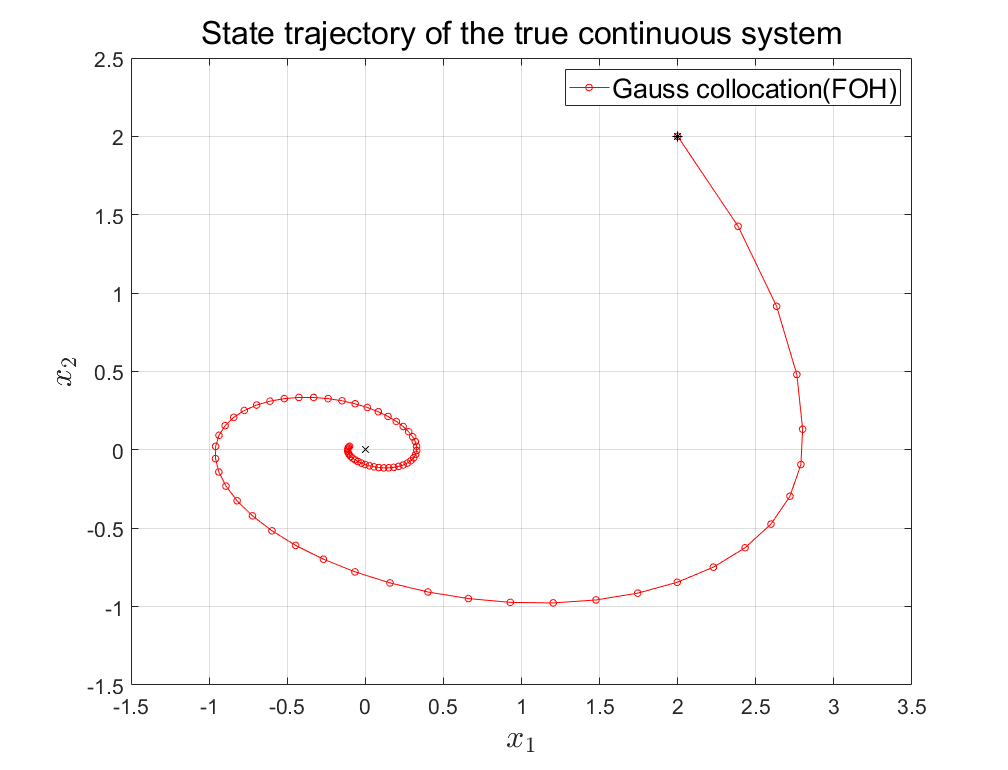
\includegraphics[width=\linewidth]{pics/gcfirst.png}
		\caption{State trajectory of the true continuous system for FOH}
		\label{fig:gcfirst.png}
	\end{subfigure}
	\hfill
	\begin{subfigure}[b]{0.37\textwidth}
		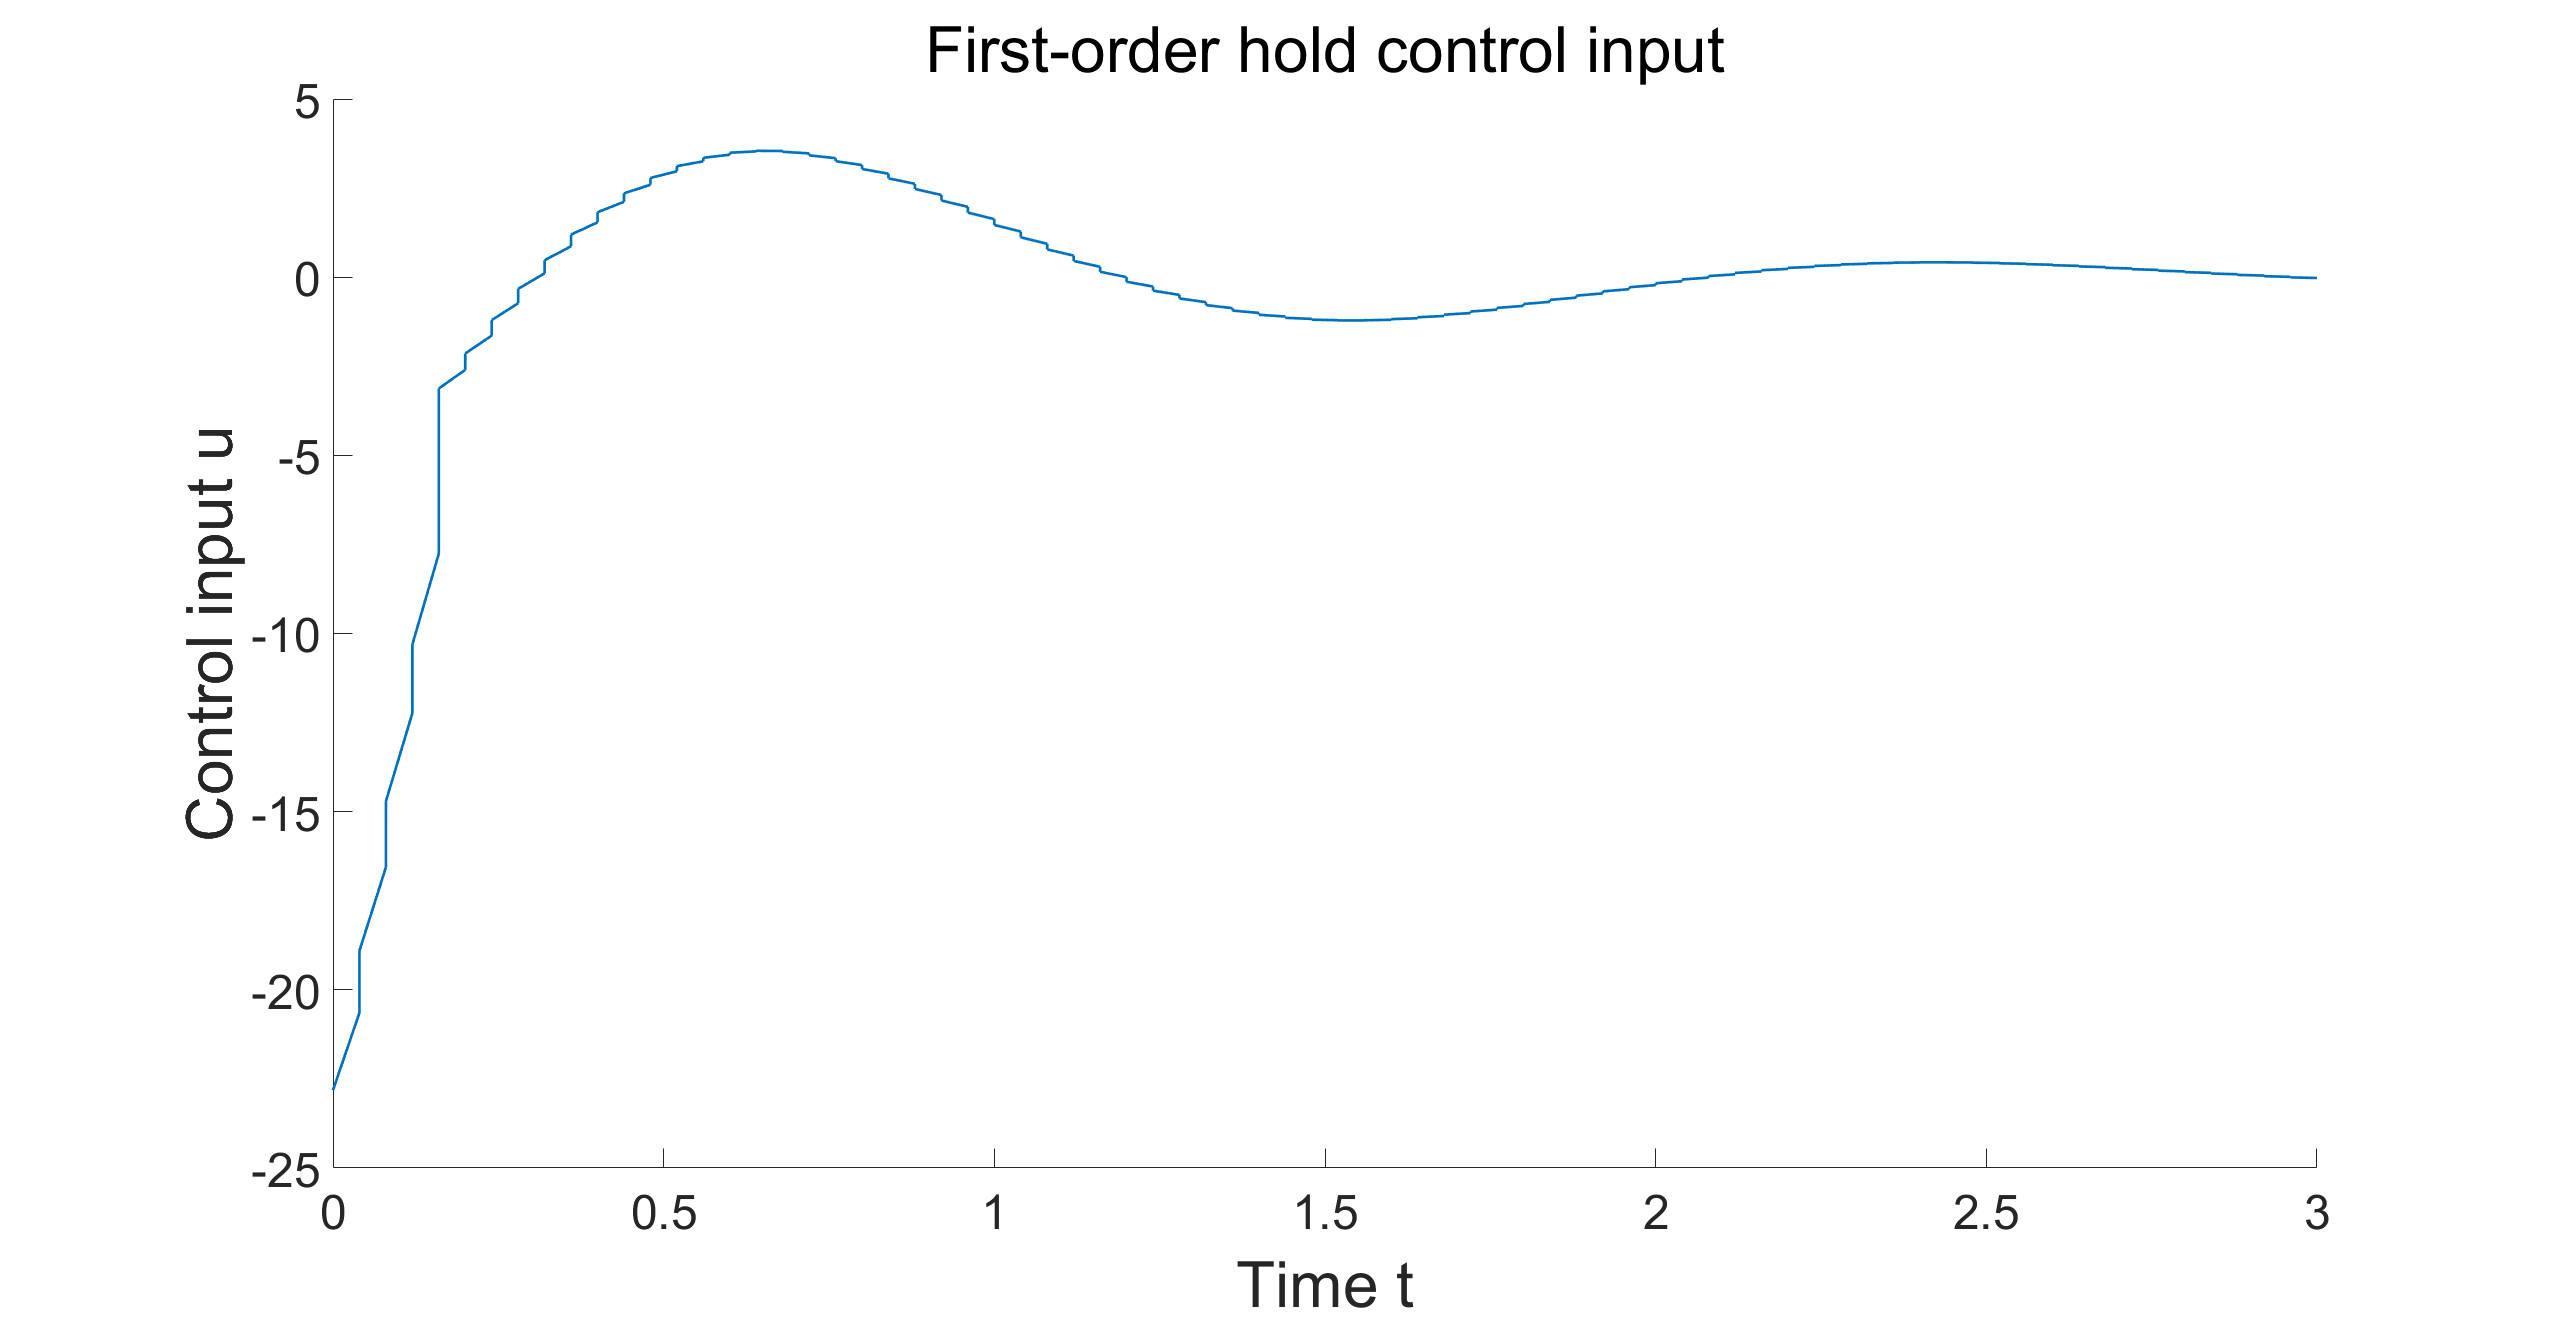
\includegraphics[width=\linewidth]{pics/FOHINPUT.png}
		\caption{FOH control input}
		\label{fig:FOHINPUT}
	\end{subfigure}
	\caption{The state trajectory and ZOH control input}
	\label{fig:The FOH}
\end{figure}
Next, we investigate the control invariant set in case of ZOH and FOH. Fig. \ref{fig:gsconinvset} shows the control invariant set in the case of ZOH control input and FOH control input. It is obvious that the control invariant set of ZOH is a subset of the control invariant set of FOH, which indicates that the MPC solver can find piecewise linear input signals for the whole state set regarding control invariance, while in the case of piecewise constant input signals (ZOH), the control invariant set is decreased.
\begin{figure}[H]
	\centering
	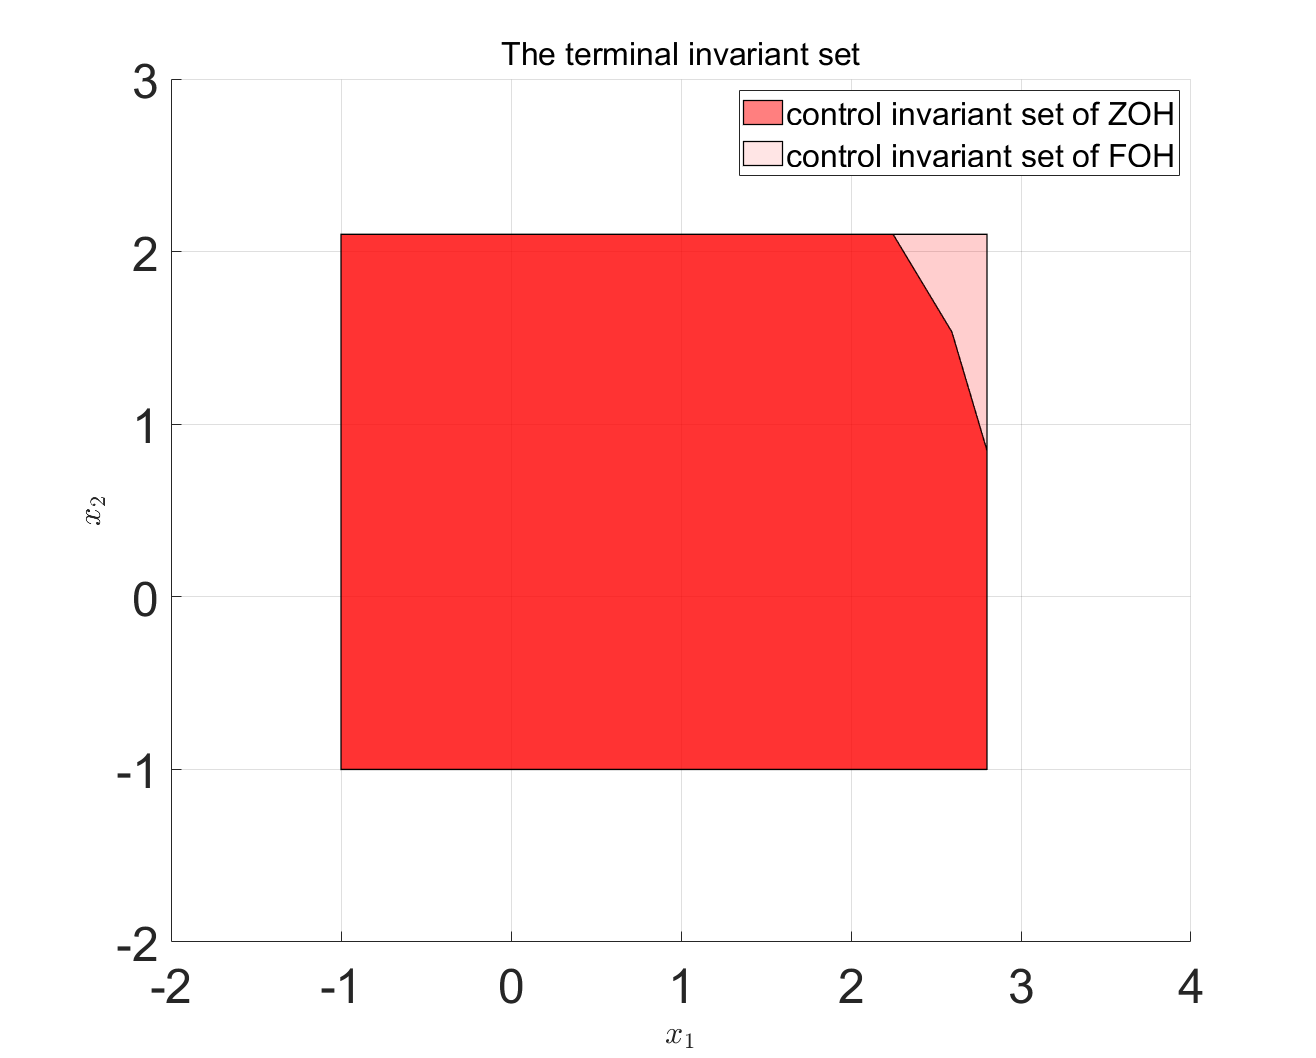
\includegraphics[width=\linewidth]{pics/gcinvariantset.png}
	\caption{The control invariant set}
	\label{fig:gsconinvset}
\end{figure}

 







%_____Zusammenfassung, Ausblick_________________________________
\chapter{Conclusion}
In this work, we compared different discretization methods for a LTI continuous time system. Specifically, we have investigated RK methods of different order and Gauss collocation methods that allow piecewise polynomial input functions within MPC. We have found that the prediction accuracy and closed-loop performance of MPC increased with increasing order of the RK method that is used for discretizing the continuous-time system model. Our simulation example also showed that we can achieve similar accuracy between RK1 with small sampling time and RK4 with large sampling time, however, this yields increased computational cost due to the increased number of optimization variables. For the Gauss collocation method, we investigated the state trajectory for different-order hold control input. It was shown that the control invariant set of FOH control input is larger than ZOH control input, as FOH can consider more input shapes than ZOH.


For future research and further extension, we  can do the same investigation on nonlinear systems, considering even higher-order hold control inputs beyond FOH, e.g., second-order hold. We also found that in Fig. \ref{fig:FOHINPUT} there are big jumps at each sampling instant, it would also be interesting to investigate how to add possible continuity constraint which would be to fix the end point of one interval with the initial point of the following interval. 



%%%%%%%%%%%%%%%%%%%%%%%%%%%%%%%%%%%%%%%%%%%%%%%%%%%%%%%%%%%%%%%%%
% APPENDIX
\appendix
%_________Appendix__________________________________

% final tutorial remarks
\ifLSRITRtutorial
	\chapter{BUSTED! Last chance to actually read the HowTo-Section!}
	
%	Make sure your thesis is well structured, that each major section does what it is supposed to do, and that the whole thing hangs together. The basic structure is often as given in this template (but other structures are possible). In particular, don't think you need to have exactly as many major sections or chapters as the list implies; sometimes it makes sense to merge things, sometimes it makes sense to move things (e.g., the literature review is in many papers deferred until after the results), sometimes it makes sense to split a logical part into several individual sections. Just use some common sense.
%	
%	Hand in your thesis at minimum \textbf{one week} before the deadline for correction. You will receive feedback for the final version and very likely have to do minor or major revisions of your writing. Plan your writing schedule to allow for these adjustments, which can have quite some impact on your grade! 
%	
%	\optional{Please have a look on our \href{https://wiki.lsr.ei.tum.de/thesiswriting_students}{thesis-guidelines} as well before submitting your \emph{final} thesis.}
	
\optional{Do not forget to check our \href{https://wiki.tum.de/display/lsritr/Students}{\underline{thesis-guidelines}} before submitting your \emph{final} thesis.}	
	
%	\section{Style and Expressions}
%	
%	Before handing in your thesis, even for an intermediate review, please perform a spellcheck and correct grammar mistakes. The report is not meant to be a narrative text. Please stick to neutral and technical style and avoid subjective or biased expressions or adjectives/adverbs such as \emph{obviously, always, very, especially well, actually, so-called etc}. Scientific writing is about precision and you should underpin your statements factually, not soften them with unnecessary qualifiers.
%	
%	... Okay enough. But please check chapter \ref{sec:Tutorial} before starting with your report. 

\section{Spellcheck reminder}
Before handing in your thesis, even for an intermediate review, please perform a proper spellcheck and correct grammar mistakes. Otherwise, there is a high likelihood that your supervisor will return your report immediately without making any comments.
\fi
% LIST OF FIGURES
\cleardoublepage
\phantomsection
\addcontentsline{toc}{chapter}{\listfigurename} 
\listoffigures 	
% LIST OF FIGuRES
\cleardoublepage
\phantomsection
\addcontentsline{toc}{chapter}{\listtablename} 
\listoftables	
% ACRONYM & NOTATIONS
% --> see include/gloss.tex
\ifdefined\AddMyGloss
    \AddMyGloss 
\fi
% BIBLIOGRAPHY
\cleardoublepage
\phantomsection
\addcontentsline{toc}{chapter}{Bibliography}
\bibliography{./refs/mybib}
\bibliographystyle{alphaurl}
% LICENSE 
\cleardoublepage
\chapter*{License}
\markright{LICENSE}
This work is licensed under the Creative Commons Attribution 3.0 Germany
License. To view a copy of this license,
visit \href{http://creativecommons.org/licenses/by/3.0/de/}{http://creativecommons.org} or send a letter
to Creative Commons, 171 Second Street, Suite 300, San
Francisco, California 94105, USA.
% TODO LIST
% this MUST be empty and/or removed in the final version of course!
\listoftodos
\end{document}
